\documentclass[journal]{IEEEtran}

%% IEEE Transactions on Industrial Informatics (TII)
%% Double-blind review — author information included below but
%% should be removed or anonymised for the review submission PDF.

\usepackage[T1]{fontenc}
\usepackage[utf8]{inputenc}
\usepackage{microtype}
\usepackage{xspace}
\usepackage{graphicx}
\usepackage{subcaption}
\usepackage{booktabs}
\usepackage{multirow}
\usepackage{amsmath}
\usepackage{amssymb}
\usepackage{array}
\usepackage{url}
\usepackage{xcolor}
\usepackage{enumitem}
\usepackage{hyperref}
\usepackage[capitalise,nameinlink]{cleveref}
\usepackage{cite}

%% TikZ / PGF for diagrams
\usepackage{tikz}
\usetikzlibrary{arrows.meta, positioning, shapes.geometric, fit, calc, backgrounds, decorations.pathreplacing}
\usepackage{pgfplots}
\pgfplotsset{compat=1.18}

\begin{document}

\title{Online Context-Aware LLM Man-in-the-Middle Attacks on CPS}

%% --- Author block (comment out for double-blind review) --------------------
\author{Huan~Bui
  and~Chenglong~Fu% <-this % stops a space
  \thanks{H.~Bui and C.~Fu are with the Department of Electrical and Computer
    Engineering, University of North Carolina at Charlotte, Charlotte, NC 28223,
    USA. E-mail: \{hbui11, cfu6\}@charlotte.edu.}%
  \thanks{Corresponding author: Huan Bui.}%
}
%% ---------------------------------------------------------------------------

\maketitle

\begin{abstract}
Large language models (LLMs) are increasingly explored for cyber-physical systems (CPS) security, yet most existing efforts either analyse static datasets, use LLMs only for offline advisory tasks, or evaluate model behaviour without a realistic closed-loop execution environment. This makes it difficult to study whether LLM-driven attack and defence strategies remain effective when exposed to real controller timing, process dynamics, and safety constraints.

This paper presents \textbf{CPSForge}, a closed-loop LLM red-team/blue-team testbed for cyber-physical systems. CPSForge is built around a real hardware-in-the-loop environment consisting of a Siemens S7 PLC programmed in TIA Portal~v17 and connected to Factory~I/O as the physical-process emulator. The framework supports two operational modes: a \emph{batch mode} in which scripted, random, or LLM-based attackers execute structured attack actions through an orchestrated pipeline, and a \emph{live agent mode} in which an autonomous LLM attacker agent and an LLM defender agent operate concurrently as independent processes, with a coordinator mediating all PLC writes through a runtime safety shield. In both modes, every proposed write is validated against configurable safety rules before reaching the PLC, and all execution is logged for reproducible analysis.

We evaluate CPSForge across three Factory~I/O scenes of increasing complexity using four attacker variants---scripted, random, LLM batch, and LLM agent---paired with threshold-based, invariant-based, and LLM-based defenders. Across 55~evaluation runs totalling 4{,}465~live PLC steps, results demonstrate that all attacker variants produce process-valid actions with 100\% execution success, the safety shield blocks only out-of-range random perturbations while permitting all well-formed attacks, and threshold/invariant detectors achieve perfect recall (1.0) across batch-mode configurations. Agent-mode experiments reveal that small local LLMs (3.8B parameters) are insufficient for reliable structured CPS agent operation, establishing a practical lower bound on model capacity for this task. To our knowledge, CPSForge is the first framework to combine LLM-driven attack generation, an autonomous LLM defender, a configurable runtime safety shield, and closed-loop adaptation, all executing against a real PLC in a hardware-in-the-loop setting.
\end{abstract}

\begin{IEEEkeywords}
cyber-physical systems, industrial control systems, large language models, man-in-the-middle attacks, context ablation, model fine-tuning, anomaly detection, runtime safety, PLC-in-the-loop
\end{IEEEkeywords}

\section{Introduction}

Cyber-physical systems (CPS) tightly integrate computation, communication, and physical processes. Industrial PLCs continuously exchange actuator commands, sensor readings, and setpoints with connected machines over field protocols such as Siemens S7, Modbus, and OPC-UA. This control-plane communication stream is the operational nervous system of an industrial plant: every polling cycle carries the commands that move valves, start conveyors, and adjust setpoints.

\textbf{Problem.} An adversary with protocol-level network access to a PLC can read this stream, infer the current process state, and inject writes timed to cause physical damage — overflowing a tank, missort items on a conveyor, or triggering a safety alarm. A defender watching the same stream can detect writes that are semantically inconsistent with the observed controller behavior and block them before they execute. Yet most LLM-for-CPS security studies remain offline or simulation-only. For example, AttackLLM~\cite{ahmed2025attackllm} evaluates generated attacks on static traces, and autonomous cyber agents such as PentestGPT~\cite{deng2024pentestgpt} and Hackphyr~\cite{rigaki2024hackphyr} focus on IT infrastructure rather than physics-constrained communication streams. Adaptive frameworks such as Evo-Defender~\cite{hu2025evodefender} study attacker--defender co-evolution but do not incorporate LLM reasoning, while MALF~\cite{ning2025malf} operates at protocol level rather than process level. As a result, it remains unclear whether LLMs can perform effective security analysis of live control-plane communication --- where decisions must account for real controller timing, process phase, and the physical consequences of each write.

\textbf{Motivation and insight.} The live communication stream between PLC and plant carries exactly the information needed for both attack and defense reasoning: current sensor values, actuator states, setpoints, and control trends. Our key insight is that by placing a local LLM as a man-in-the-middle agent in this stream --- reading the same tags an attacker or defender would observe --- we can automate both roles systematically and symmetrically on real hardware. The same model, same observation pipeline, and same context structure serve as both red team and blue team, differing only in the prompt and the action they take.

\textbf{How we solve it.} We propose \textbf{CPSForge}, a framework that places a local LLM as a man-in-the-middle agent in real PLC communication, automating both red team (attack injection) and blue team (write interception) on the live tag stream. Every 500\,ms, CPSForge reads the PLC tag stream via S7 protocol (python-snap7). Every three polling cycles, it assembles a context-tier-specific prompt from the observed communication data and queries the LLM: as red team, decide to \emph{attack} (inject a write) or \emph{wait}; as blue team, decide to \emph{allow} or \emph{block} a proposed write. All writes are mediated by a mandatory safety shield before reaching the PLC. The framework is configuration-driven: the scene YAML provides the semantic interpretation of the tag stream (tag descriptions, valid ranges, attack surface, control objectives) for each plant. Connecting a different plant --- water treatment, power grid substation, manufacturing line --- requires only a new scene YAML; no code changes are required. We evaluate CPSForge on three Factory~I/O scenes connected to a real Siemens S7-1200 PLC.

Accordingly, the primary scientific contributions of this work are:

\begin{itemize}[leftmargin=1.5em]
    \item \textbf{C1.~Closed-loop LLM red team on live PLC communication.} We introduce an online LLM agent that operates as a man-in-the-middle in the PLC control loop: observe plant state $\to$ infer process phase $\to$ build context $\to$ decide (attack$|$wait) $\to$ act $\to$ observe result. Prior LLM-based CPS attack work either generates attacks offline without executing them (AttackLLM~\cite{ahmed2025attackllm}), operates at the network-packet layer rather than process-level tags (MALF~\cite{ning2025malf}), or targets IT infrastructure rather than physics-constrained control streams (PentestGPT~\cite{deng2024pentestgpt}). HARVEY~\cite{garcia2017harvey} demonstrated closed-loop PLC MitM but required a hand-crafted physics model per plant. CPSForge replaces plant-specific models with general-purpose LLM reasoning plus a configuration-driven scene abstraction, enabling the same agent to attack different plants without code changes.
    \item \textbf{C2.~Context-ablation study linking adversary knowledge to attack capability.} We define three strictly controlled context tiers---minimal (tag values only), partial (values + history + descriptions), and full (+ phase inference + prior action effects + attack guidance)---that map to realistic adversary reconnaissance levels: passive eavesdropping, field-device enumeration, and full plant documentation access. This enables the first controlled measurement of the \emph{minimum} process knowledge an LLM adversary needs to mount effective CPS attacks---a question that prior LLM-for-CPS work has not isolated because it evaluates only a single (typically maximal) context configuration.
    \item \textbf{C3.~Dual-objective fine-tuning study.} We design a QLoRA fine-tuning pipeline that trains Qwen2.5-3B-Instruct on 2{,}057~examples covering both verified successful attack traces and defense decisions (block/allow). Unlike Hackphyr~\cite{rigaki2024hackphyr}, which fine-tunes for IT penetration testing only, our dual-objective training enables a controlled before/after comparison of how task-specific CPS training changes \emph{both} red team and blue team capability within the same model---testing whether attack-aware fine-tuning transfers to defense.
    \item \textbf{C4.~Symmetric LLM blue team with defense comparison.} We propose an LLM-based blue team agent that uses the \emph{same model architecture, context pipeline, and inference infrastructure} as the red team, creating a symmetric attacker--defender pairing on the live tag stream. Unlike Evo-Defender~\cite{hu2025evodefender}, which co-evolves non-LLM strategies on simulators, and LLM-based IDS approaches~\cite{ann2024ids_llm, sharshar2025explainable} that classify historical traffic logs, our LLM defender evaluates each proposed PLC write in real time before execution. We compare seven defense configurations---no defense, rule-based (threshold, phase-aware, intent-consistency), LLM-only, and combined---enabling the first systematic comparison of rule-based vs.\ LLM-based vs.\ hybrid runtime defense against LLM-generated CPS attacks.
    \item \textbf{C5.~Cross-model robustness evaluation.} We evaluate three local models from two families---Qwen2.5-3B-Instruct, Qwen3-1.7B, and SmolLM3-3B---to test whether observed attack and defense trends are robust across architectures or strongly model-specific.
    \item \textbf{C6.~Frontier model scaling study.} We extend the evaluation with GPT-4o-mini (a frontier API model) across the same three scenes, demonstrating that self-deterrence vanishes at frontier scale, ASR reaches 100\% on Sorting by Weight, and the local LLM defender generalizes cross-model to block frontier-model attacks.
    \item \textbf{C7.~Comprehensive PLC-in-the-loop evaluation.} We evaluate C1--C6 through 333~live experiment runs across three Factory~I/O scenes on a real Siemens S7-1200 PLC, with $\geq$3~repeats per cell and unified per-step logging for reproducibility.
\end{itemize}

The remainder of the paper is organized as follows. Section~\ref{sec:background} provides background and motivation. Section~\ref{sec:threat} defines the threat model and assumptions. Section~\ref{sec:design} presents the CPSForge architecture. Section~\ref{sec:implementation} describes the implementation over a real PLC and Factory~I/O. Section~\ref{sec:methodology} describes the evaluation methodology. Section~\ref{sec:evaluation} presents experimental results. Section~\ref{sec:discussion} discusses findings and limitations. Section~\ref{sec:related} reviews related work, and Section~\ref{sec:conclusion} concludes.

\section{Background and Motivation}
\label{sec:background}

\subsection{Cyber-Physical Systems and Industrial Control}

Cyber-physical systems combine software control, networked communication, and physical dynamics. In industrial automation, PLCs serve as the primary control components that execute ladder logic or structured text, interact with sensors and actuators, and enforce operational sequences. The correctness of such systems depends not only on software behavior, but also on scan timing, process feedback, interlocks, and safety thresholds.

Compared to traditional IT environments, CPS attacks are constrained by the physical process. A successful adversary must reason about actuator timing, sensor semantics, controller state, and process dependencies. Similarly, effective defense must consider more than network traces or software logs; it must also account for physical behavior and unsafe state transitions.

\subsection{Why LLMs Matter in CPS Security}

LLMs offer flexible reasoning over unstructured descriptions, structured telemetry, process semantics, and attacker objectives. Recent work has shown that they can generate process-aware attacks~\cite{ahmed2025attackllm}, synthesize invariants~\cite{fakih2024llm4plc}, and support security analysis~\cite{xu2024llm_cybersec_survey}. However, LLMs also introduce well-known risks: they can hallucinate, over-generalize, misinterpret context, or propose unsafe actions. These risks are amplified in CPS because model outputs may influence physical behavior.

Therefore, the research question this paper addresses is whether LLM reasoning can be embedded into a rigorously constrained environment where actions are structured, validated, logged, and evaluated against real process behavior---and whether the resulting framework yields insights that purely offline or simulated evaluations cannot.

\subsection{Limits of Existing Evaluation Practice}

Much of the current CPS security literature relies on benchmark datasets, offline detection experiments, or scripted attack scenarios. While these methods are useful, they do not fully capture the interaction between a live controller, evolving plant state, and actuation decisions. Offline traces cannot reproduce real controller scan cycles, online state transitions, or the consequences of repeated attack attempts.

Likewise, recent LLM-based CPS studies often stop at anomaly explanation, invariant extraction, or attack ideation. Without a closed-loop execution environment, it remains unclear whether LLM-generated strategies are actually process-valid, whether they survive practical constraints, and whether defenses improve meaningfully after exposure to such attacks.

\subsection{Motivation for a Closed-Loop Testbed}

CPSForge is motivated by the need for a realistic yet safe experimental platform that can study offensive and defensive LLM use together. The real PLC provides authentic controller timing and execution semantics, while Factory~I/O supplies reproducible software-emulated industrial process scenes with realistic I/O behaviour. This combination---which we term \emph{PLC-in-the-loop}---provides a practical substrate that reproduces real controller scan cycles and actuator response while keeping the physical process safely virtualised. Unlike full hardware-in-the-loop testbeds with real sensors and actuators (e.g., SWaT~\cite{mathur2016swat}), this configuration cannot capture physical coupling effects such as fluid dynamics or mechanical wear, but it preserves the most security-relevant aspect: the PLC executes real control logic on each scan cycle and the process emulator responds with physically plausible state transitions.

The design also emphasizes a closed-loop attacker-defender cycle. A one-shot attacker evaluation reveals only whether a particular defense succeeds on a fixed set of cases. In contrast, a closed-loop system can reveal how defenders fail, how attacks diversify, and whether repeated adaptation improves resilience. This aligns more closely with real-world adversarial evolution and provides a stronger foundation for research claims about robustness.

\subsection{Design Goals}

The design of CPSForge is guided by four main goals:

\begin{itemize}[leftmargin=1.5em]
    \item \textbf{Realism.} The system should operate over a real PLC and a live process emulator rather than relying solely on offline traces or purely synthetic controllers.
    \item \textbf{Safety.} No model or attack component should write directly to the controller without mediation by a safety layer.
    \item \textbf{Reproducibility.} Every experiment should produce structured artifacts that support replay, auditing, and analysis.
    \item \textbf{Adaptation.} The framework should support repeated attack and defense rounds so that defender improvement can be measured over time.
\end{itemize}
\section{Threat Model and Assumptions}
\label{sec:threat}

This section defines the threat model, the role of the LLM attacker, the defender assumptions, and the safety boundaries enforced by CPSForge.

\subsection{Adversary Goals}

The adversary aims to manipulate the cyber-physical process in a way that causes measurable impact while remaining process-valid and, when possible, difficult to detect. Depending on the scene, impact may include unsafe state transitions, degraded performance, incorrect sequencing, product handling failures, or violations of expected operational behavior. The adversary may also seek to delay or evade detection by maintaining plausible sensor and actuator patterns.

\subsection{Adversary Capabilities}

The attacker in CPSForge models a post-compromise adversary who has achieved S7 protocol-level network access to the PLC control network --- for example, through credential theft, insider access, exploitation of an engineering workstation, or lateral movement from the IT network. This access level is realistic: S7 communication between PLC and SCADA/HMI systems is commonly exposed on flat industrial networks, and tools such as python-snap7 allow any network-reachable host to read and write PLC data blocks without authentication on many deployed systems.

With S7-level access, the adversary can: (i)~continuously read the live tag stream (sensor values, actuator states, setpoints) at polling rate; (ii)~infer the current operational phase from tag value patterns; (iii)~inject writes to any writable tag in the PLC data block. Rather than modeling raw memory addresses or firmware-level access, CPSForge expresses attacks at the process-semantic level --- the same level at which a process engineer or SCADA operator would interact with the system. The exact attack surface (which tags are writable by the attacker) is scene-specific and explicitly configured in the scene YAML.

Within this scope, the attacker can perform actuator overrides, setpoint shifts, sensor spoofing, timing delays, and sequence perturbations --- all expressed as structured writes to the PLC tag stream.

\subsection{LLM Role}

The LLM serves as a man-in-the-middle agent in the PLC communication stream, not as a trusted controller. Every three polling cycles (1.5\,s), the LLM receives a structured snapshot of the observed tag stream (whose richness depends on the context tier) and returns a structured decision. As red team: \emph{attack} (with a complete write specification: tag, value, duration, action type) or \emph{wait}. As blue team: \emph{allow} or \emph{block} a proposed write, with a suspicion score and reasoning.

The LLM does not directly access PLC memory, bypass process interlocks, or issue unrestricted writes. All LLM outputs are treated as untrusted proposals until validated by the safety shield. The shield enforces tag whitelists, value ranges, duration caps, and process invariants before any write reaches the PLC.

This architecture separates LLM reasoning capability (which we evaluate) from execution privilege (which is strictly bounded). The paper evaluates how useful LLM communication-analysis outputs are under varying context depths (RQ1), whether training on real communication traces improves those outputs (RQ2), and whether online stream feedback is necessary (RQ3).

\subsection{Timing Model and Latency Characterization}
\label{sec:threat:timing}

CPSForge does \emph{not} operate at the PLC scan-cycle timescale (${\sim}$1--10\,ms). LLM inference on the 3B model takes 13--33\,s per call depending on prompt length and context tier. Each LLM call is issued every three polling cycles (1.5\,s of observation time); during inference, polling continues but no new attacker decisions are made until the call returns. Total wall-clock time per 60-step run is 6--10~minutes.

This latency profile positions the LLM adversary as a \emph{supervisory-timescale} attacker---analogous to an operator or SCADA engineer making strategic process interventions at multi-second intervals---not a sub-millisecond PLC-level manipulator. This is a realistic and well-documented threat model: documented ICS incidents operate on timescales far longer than the PLC scan cycle. The Stuxnet campaign manipulated centrifuge speeds over weeks~\cite{langner2011stuxnet}, the 2015 Ukrainian grid attack coordinated breaker openings over approximately 30~minutes~\cite{liang2017ukraine}, and the TRITON/TRISIS attack on safety instrumented systems required multi-hour reconnaissance before a single write~\cite{johnson2017triton}. Even the fastest known ICS MitM attacks (e.g., HARVEY~\cite{garcia2017harvey}) operate at control-loop timescales (${\sim}$100\,ms--1\,s), not PLC scan-cycle speeds.

Our 30-second observation window with up to 10 strategic writes is conservative relative to real-world ICS attack timelines, where adversaries typically have persistent access over hours or days. The 10-attack budget tests whether the LLM can \emph{select the right writes} from limited opportunities---a harder task than unrestricted injection. This budget also keeps experiments within Factory~I/O's process cycle time (most sorting sequences complete in 20--40\,s), ensuring each run observes at least one complete operational cycle.

\subsection{Defender Model}

The defender has access to the observed plant state, controller state, alarms, and experiment telemetry collected from the PLC-process loop. Depending on the detector configuration, the defender may use static thresholds, process invariants, or learned sequence models. The defender does not assume oracle knowledge of the attacker’s true intent, though logged attacks can later be used for offline analysis and adaptation.

The defender is evaluated on its ability to detect process deviations, unsafe states, suspicious sequences, or other operational anomalies caused by the attacker.

\subsection{Safety Boundary and Trusted Components}

CPSForge assumes that the safety shield is part of the trusted computing base for experimentation. The shield is responsible for validating every candidate action before it reaches the PLC. In practice, it enforces writable-tag whitelists, legal value ranges, maximum override durations, cooldown periods, forbidden simultaneous actions, and scene-specific safety invariants.

The real PLC, deployed logic, and scene configuration are also assumed to be correctly installed and maintained by the operator. Human supervision remains in scope, and the framework assumes that emergency-stop and reset procedures are available during live experiments.

\subsection{Scope and Limitations}

The present work does not model arbitrary firmware compromise, PLC root access, or unrestricted malicious code deployment. The attacker operates within a configured action space mediated by the safety shield, which bounds all writes to process-safe ranges. This bounded model is a deliberate design choice: it enables safe, repeatable, and auditable experimentation while still permitting the attacker to cause measurable process impact---as the evaluation demonstrates. However, this means experimental attack success rates reflect effectiveness \emph{within the configured envelope}, not the full capability of an unconstrained adversary. The framework is designed to study whether LLMs can produce process-grounded attack strategies and whether defenders can improve under such pressure; it does not claim to replicate the full scope of nation-state ICS attack campaigns.

\subsection{Extended Threat Model: Three Attack Tiers}
\label{sec:threat:tiers}

While the original evaluation focuses on I/O-level data manipulation (Tier~1), we extend the threat model to capture the full spectrum of PLC-level attacks observed in real-world incidents. This multi-tier model positions CPSForge's contributions within a broader taxonomy and motivates two additional testbeds.

\subsubsection{Tier 1: I/O Data MitM (Original Evaluation)}
The attacker reads and writes PLC I/O tags (sensors, actuators, setpoints) via S7 protocol. Written values are \emph{overwritten by PLC logic each scan cycle}, requiring continuous or precisely timed injection. This tier maps to the Online MITM Attacker (\S\ref{sec:design}) and covers all 333~runs in the evaluation. Real-world analogues include Oldsmar (single setpoint write), BlackEnergy (breaker commands via SCADA HMI), and Industroyer (automated protocol-level commands)---see Table~\ref{tab:incidents} in \S\ref{sec:background:incidents}.

\subsubsection{Tier 2: Deep State Manipulation (New)}
The attacker targets \emph{internal PLC state variables}---state machine indices (\texttt{iState}), timers, classification flags, thresholds, and enable bits---that are accessible via the same S7 protocol but are \textbf{never refreshed by PLC logic}. Unlike Tier~1 writes that the PLC immediately overwrites, a single Tier~2 write to a variable like \texttt{Enable} (BOOL) or \texttt{LightThresh} (REAL) persists indefinitely until the scene resets, because the PLC reads but never re-initializes these variables during normal operation.

This tier is analogous to Stuxnet's writes to DB890, which modified PLC behavior by changing data block values rather than modifying the PLC program itself~\cite{langner2013kill}. The key insight is that \emph{behavioral modification} of a PLC can be achieved through data alone---by targeting internal state variables that the control logic trusts implicitly.

We implement this tier as the \emph{DeepStateMITMAttacker}, which shares the same observation--phase--context--decide--act loop as the Tier~1 attacker but operates on an extended attack surface (\texttt{deep\_state\_attack\_surface} in the scene YAML) with eight attack categories: threshold manipulation, state machine jump, timer acceleration, safety kill switch, decision flag spoofing, setpoint hijack, counter spoofing, and mode manipulation.

The primary defense for this tier is the \emph{StateConsistencyChecker}, which enforces state transition validity (e.g., \texttt{iState} can only advance to adjacent states), timer progression bounds, protected variable guards (e.g., \texttt{Enable} is never writable during operation), and classification flag phase-locking.

\subsubsection{Tier 3: Logic Code Generation (New)}
The attacker analyzes PLC control logic (SCL source code) and generates adversarial modifications---minimal, compilable code changes designed to disrupt the process while remaining difficult to detect through code review. This tier requires engineering workstation access for deployment (manual TIA Portal upload) and tests the LLM's \emph{cognitive capability} to comprehend and weaponize structured control logic.

This maps directly to Stuxnet's offline payload development methodology: the attack payload (modified OB1/OB35) was crafted by analyzing centrifuge control logic, then deployed via USB~\cite{falliere2011w32}. The LLM's contribution is the same \emph{analysis and generation} step; deployment is out of scope.

The \emph{LogicAnalyzer} scans SCL source for seven vulnerability categories (dead code injection, comparison inversion, timer alteration, interlock removal, gradual drift, state shortcut, sensor clamping) and generates minimal adversarial code modifications with stealth assessments and detection difficulty ratings. The symmetric defense, \emph{CodeReviewDefender}, reviews SCL diffs using the same LLM architecture and outputs approve/reject decisions with suspicion scores.

\subsubsection{LLM-Accessible Attack Surface Enumeration}
\label{sec:threat:attack_surface}

A central question for LLM-enabled CPS attacks is: \emph{what can the model actually reach?} Table~\ref{tab:attack_surface} enumerates the concrete variables accessible via S7 protocol across our three evaluation scenes. All variables reside in non-optimized PLC data blocks (DBs), which python-snap7 can read and write by byte offset without authentication on default S7-1200 configurations.

\begin{table}[h]
\centering
\caption{LLM-accessible attack surface per scene. ``PLC refresh'' indicates whether the PLC overwrites the variable each scan cycle ($\checkmark$) or trusts the stored value ($\times$).}
\label{tab:attack_surface}
\small
\begin{tabular}{@{}llllc@{}}
\toprule
\textbf{Scene} & \textbf{Variable} & \textbf{Type} & \textbf{Attack Category} & \textbf{PLC Refresh} \\
\midrule
\multirow{4}{*}{\shortstack[l]{Level\\Control}} & SetpointIn & REAL & Setpoint hijack & $\times$ \\
& FillValve & REAL & Actuator override & $\checkmark$ \\
& DischargeValve & REAL & Actuator override & $\checkmark$ \\
& Enable & BOOL & Safety kill & $\times$ \\
\midrule
\multirow{5}{*}{\shortstack[l]{Sorting\\Weight}} & LightThresh & REAL & Threshold manip. & $\times$ \\
& HeavyThresh & REAL & Threshold manip. & $\times$ \\
& iState & INT & State machine jump & $\checkmark$ \\
& Conveyor1/2/3 & BOOL & Actuator override & $\checkmark$ \\
& Sorter1/2 & BOOL & Actuator override & $\checkmark$ \\
\midrule
\multirow{5}{*}{\shortstack[l]{Sorting\\Height}} & iState & INT & State machine jump & $\checkmark$ \\
& TurnTimer & INT & Timer acceleration & $\checkmark$ \\
& DwellTimer & INT & Timer acceleration & $\checkmark$ \\
& Enable & BOOL & Safety kill & $\times$ \\
& IsTall & BOOL & Decision flag spoof & $\checkmark$ \\
\bottomrule
\end{tabular}
\end{table}

The distinction between PLC-refreshed ($\checkmark$) and non-refreshed ($\times$) variables is critical. \textbf{Tier~1 attacks} target refreshed variables, requiring the attacker to re-inject each scan cycle or time the injection precisely between PLC writes. \textbf{Tier~2 attacks} target non-refreshed variables, where a single write persists until explicit reset. This analysis demonstrates that even simple PLC programs contain \emph{semantic trust assumptions}---variables like \texttt{SetpointIn}, \texttt{Enable}, and classification thresholds are read by the control logic on every scan but are never re-initialized, creating persistent write targets. This finding generalizes to real-world PLCs, where data block parameters (alarm limits, recipe values, PID tuning constants) are typically writable via the same protocol used for process data, with no access control distinction~\cite{mclaughlin2016cps_integrity}.

\subsubsection{Tier Comparison}

\begin{table}[h]
\centering
\caption{Three-tier threat model comparison}
\label{tab:threat-tiers}
\small
\begin{tabular}{@{}lccc@{}}
\toprule
\textbf{Property} & \textbf{Tier 1: I/O MitM} & \textbf{Tier 2: Deep State} & \textbf{Tier 3: Logic Gen} \\
\midrule
Protocol & S7 (python-snap7) & S7 (python-snap7) & TIA Portal (manual) \\
Target & I/O tags & Internal state & PLC program \\
Persistence & 1 scan cycle & Permanent & Permanent \\
PLC overwrites? & Yes & No & N/A (is the logic) \\
Automation & Fully automated & Fully automated & Manual upload \\
Real-world & Oldsmar, Industroyer & Stuxnet DB890 & Stuxnet OB1/OB35 \\
Defense & Safety shield + LLM & State consistency & Code review \\
\bottomrule
\end{tabular}
\end{table}
\section{System Design}
\label{sec:design}

CPSForge is organised as a closed-loop CPS security framework built around six interacting layers---physical execution, observation and logging, attack generation, safety enforcement, defence, and adaptation---plus a seventh \emph{agent mode} layer that enables autonomous multi-agent operation. Figure~\ref{fig:architecture} illustrates the complete pipeline.

\begin{figure*}[t]
    \centering
    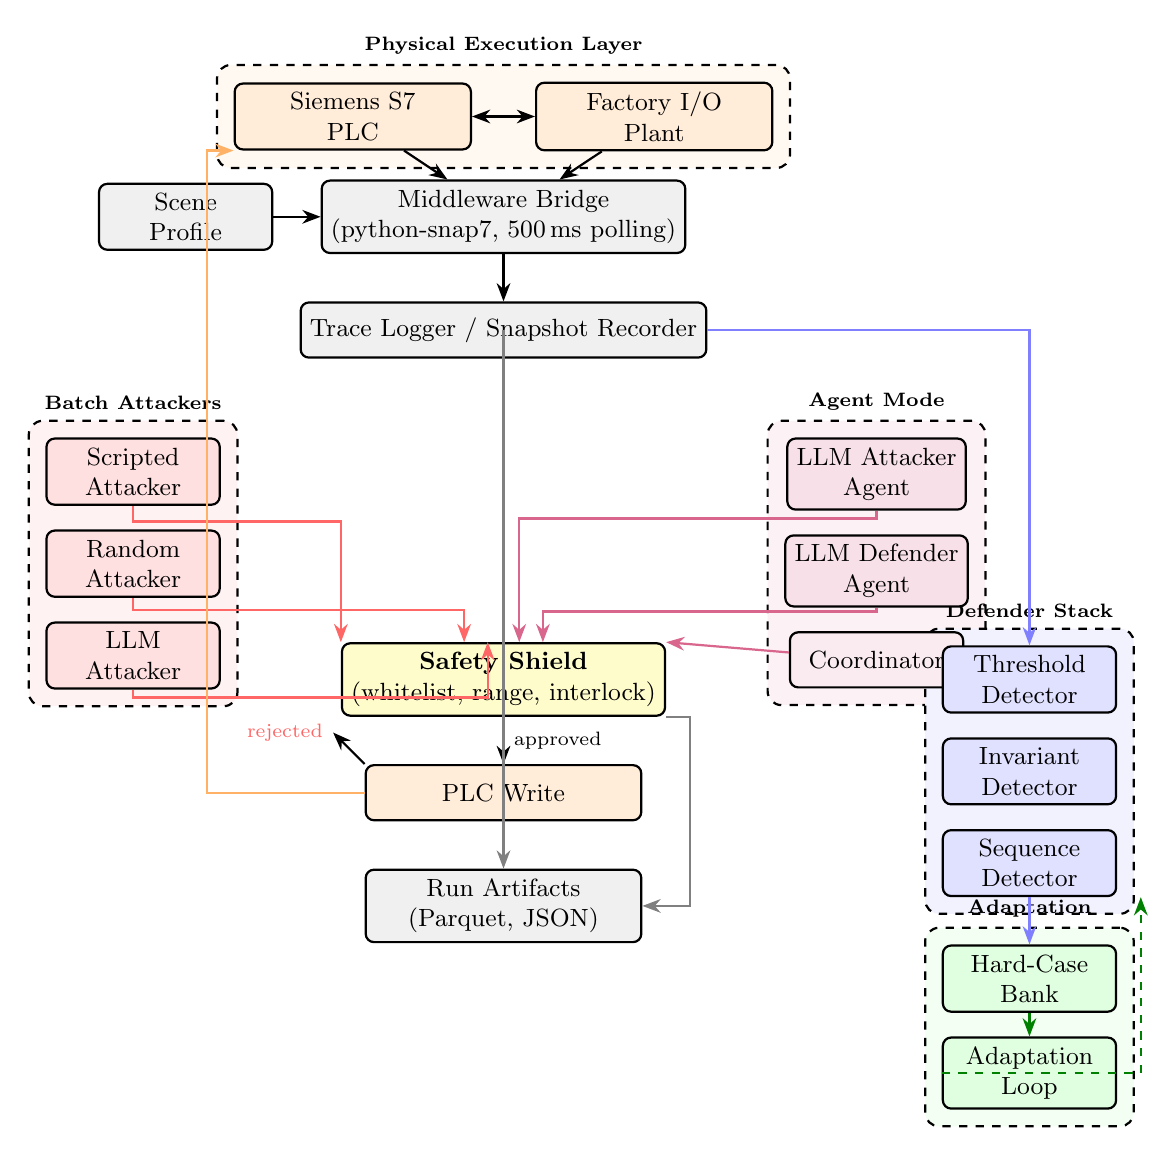
\begin{tikzpicture}[
        >=Stealth,
        node distance=0.6cm and 0.5cm,
        every node/.style={font=\small},
        layer/.style={draw, rounded corners=3pt, minimum width=2.2cm, minimum height=0.7cm, align=center, thick},
        plcbox/.style={layer, fill=orange!15, minimum width=3cm},
        atkbox/.style={layer, fill=red!12},
        shieldbox/.style={layer, fill=yellow!20},
        defbox/.style={layer, fill=blue!12},
        adaptbox/.style={layer, fill=green!12},
        logbox/.style={layer, fill=gray!12},
        agentbox/.style={layer, fill=purple!12},
        groupbox/.style={draw, dashed, rounded corners=5pt, inner sep=6pt, thick},
        arr/.style={->, thick, >=Stealth},
        darr/.style={<->, thick, >=Stealth},
    ]

    %% ===== Physical Execution Layer =====
    \node[plcbox] (plc) {Siemens S7\\PLC};
    \node[plcbox, right=0.8cm of plc] (fio) {Factory I/O\\Plant};
    \draw[darr] (plc) -- (fio);

    %% ===== Middleware / Observation =====
    \node[logbox, below=0.8cm of $(plc)!0.5!(fio)$, minimum width=4.5cm] (mw) {Middleware Bridge\\(python-snap7, 500\,ms polling)};
    \draw[arr] (plc) -- (mw);
    \draw[arr] (fio) -- (mw);

    %% ===== Scene Profile =====
    \node[logbox, left=0.6cm of mw] (scene) {Scene\\Profile};
    \draw[arr] (scene) -- (mw);

    %% ===== Trace Logger =====
    \node[logbox, below=0.6cm of mw, minimum width=4.5cm] (logger) {Trace Logger / Snapshot Recorder};
    \draw[arr] (mw) -- (logger);

    %% ===== Branch: Batch Mode (left) =====
    \node[atkbox, below left=1.0cm and 1.0cm of logger] (scripted) {Scripted\\Attacker};
    \node[atkbox, below=0.3cm of scripted] (random) {Random\\Attacker};
    \node[atkbox, below=0.3cm of random] (llmbatch) {LLM\\Attacker};

    %% ===== Branch: Agent Mode (right) =====
    \node[agentbox, below right=1.0cm and 1.0cm of logger] (atk_agent) {LLM Attacker\\Agent};
    \node[agentbox, below=0.3cm of atk_agent] (def_agent) {LLM Defender\\Agent};
    \node[agentbox, below=0.3cm of def_agent, fill=purple!8] (coord) {Coordinator};

    %% ===== Safety Shield (center) =====
    \node[shieldbox, below=3.6cm of logger, minimum width=3.5cm, minimum height=0.8cm] (shield) {\textbf{Safety Shield}\\(whitelist, range, interlock)};

    %% Arrows from attackers to shield
    \draw[arr, red!60] (scripted.south) -- ++(0,-0.2) -| (shield.north west);
    \draw[arr, red!60] (random.south) -- ++(0,-0.15) -| ([xshift=-0.5cm]shield.north);
    \draw[arr, red!60] (llmbatch.south) -- ++(0,-0.1) -| ([xshift=-0.2cm]shield.north);

    %% Arrows from agents to shield
    \draw[arr, purple!60] (atk_agent.south) -- ++(0,-0.1) -| ([xshift=0.2cm]shield.north);
    \draw[arr, purple!60] (def_agent.south) -- ++(0,-0.05) -| ([xshift=0.5cm]shield.north);
    \draw[arr, purple!60] (coord) -- (shield.north east);

    %% ===== PLC Write =====
    \node[plcbox, below=0.6cm of shield, minimum width=3.5cm] (write) {PLC Write};
    \draw[arr] (shield) -- node[right, font=\scriptsize]{approved} (write);
    \draw[arr] (write.north west) -- ++(-0.4,0.4) node[left, font=\scriptsize, text=red!60]{rejected};

    %% Arrow back to PLC
    \draw[arr, thick, orange!60] (write.west) -- ++(-2.0,0) |- (plc.south west);

    %% ===== Defenders =====
    \node[defbox, right=3.5cm of shield] (thresh) {Threshold\\Detector};
    \node[defbox, below=0.3cm of thresh] (invar) {Invariant\\Detector};
    \node[defbox, below=0.3cm of invar] (seqdet) {Sequence\\Detector};

    \draw[arr, blue!50] (logger.east) -| (thresh.north);

    %% ===== Adaptation =====
    \node[adaptbox, below=0.6cm of seqdet] (hcbank) {Hard-Case\\Bank};
    \node[adaptbox, below=0.3cm of hcbank] (adapt) {Adaptation\\Loop};
    \draw[arr, blue!50] (seqdet) -- (hcbank);
    \draw[arr, green!50!black] (hcbank) -- (adapt);
    \draw[arr, green!50!black, dashed] (adapt.west) -| ([xshift=0.3cm]seqdet.south east);

    %% ===== Artifacts =====
    \node[logbox, below=0.6cm of write, minimum width=3.5cm] (artifacts) {Run Artifacts\\(Parquet, JSON)};
    \draw[arr, gray] (logger) -| (artifacts);
    \draw[arr, gray] (shield.south east) -- ++(0.3,0) |- (artifacts.east);

    %% ===== Group boxes =====
    \begin{scope}[on background layer]
        \node[groupbox, fill=orange!5, fit=(plc)(fio), label={[font=\scriptsize\bfseries]above:Physical Execution Layer}] {};
        \node[groupbox, fill=red!5, fit=(scripted)(random)(llmbatch), label={[font=\scriptsize\bfseries]above:Batch Attackers}] {};
        \node[groupbox, fill=purple!5, fit=(atk_agent)(def_agent)(coord), label={[font=\scriptsize\bfseries]above:Agent Mode}] {};
        \node[groupbox, fill=blue!5, fit=(thresh)(invar)(seqdet), label={[font=\scriptsize\bfseries]above:Defender Stack}] {};
        \node[groupbox, fill=green!5, fit=(hcbank)(adapt), label={[font=\scriptsize\bfseries]above:Adaptation}] {};
    \end{scope}

    \end{tikzpicture}
    \caption{CPSForge system architecture. The physical PLC--Factory~I/O loop (top) feeds observations to both batch-mode attackers (left) and agent-mode LLM agents (right). All proposed writes---offensive and corrective---pass through the safety shield before reaching the PLC. The defender stack monitors process state and feeds hard cases to the adaptation loop (right).}
    \label{fig:architecture}
\end{figure*}

\subsection{Physical Execution Layer}

At the foundation of CPSForge is a live hardware-in-the-loop environment. A Siemens S7 PLC executes control logic deployed from TIA Portal~v17, while Factory~I/O emulates the physical process. This design provides realistic controller behaviour, including actual scan timing, state transitions, and control-loop interactions that are difficult to reproduce through offline logs alone.

Each process scene is represented as a scene profile containing tag metadata, process descriptions, attack surface definitions, safety rules, and reset procedures. The architecture supports both continuous-process scenes (e.g., tank level control) and discrete event-driven scenes (e.g., conveyor sorting).

\subsection{Observation and Logging Layer}

A middleware bridge continuously reads the PLC state and records structured plant snapshots. A snapshot includes sensor values, actuator states, controller mode bits, alarms, setpoints, timestamps, and experiment context. Logging is designed to be replay-ready and audit-friendly.

This layer serves several purposes. First, it provides current context for the attacker and defender. Second, it enables post~hoc analysis of attack success, physical impact, and detection behaviour. Third, it supports replay-based evaluation and adaptation.

\subsection{Attack Layer}

The attack layer supports multiple attacker types: scripted baselines, bounded random perturbation, and an LLM-based attacker. The key design decision is that attack actions are expressed in a structured semantic schema rather than as raw PLC memory writes.

Example attack categories include sensor spoofing, actuator overrides, setpoint shifts, timing delays, and sequence perturbations. An LLM attacker receives scene context, current plant state, allowed capabilities, and attacker objectives, then returns one or more structured actions. These actions are interpreted as candidate plans, not automatically executed commands.

\subsection{Safety Shield}

The safety shield is the central enforcement mechanism in CPSForge. Every attack action, regardless of source, must pass through the shield before being translated into live writes. The shield evaluates whether the target is writable, whether the value is within configured limits, whether the duration is acceptable, and whether the proposed action conflicts with interlocks or scene-specific invariants.

The shield can approve, reject, or normalise an action. It also records the reasoning behind each decision and can generate rollback plans or expiration timers. This layer allows the framework to study attack behaviour while preserving operator-defined safety boundaries. In agent mode, the shield additionally evaluates \emph{corrective} writes proposed by the defender agent, applying the same safety constraints to defensive actions.

\subsection{Defender Layer}

The defender layer monitors the plant state during execution and emits alerts when anomalous or unsafe behaviour is detected. CPSForge supports multiple detector families:

\begin{itemize}[leftmargin=1.5em]
    \item threshold-based detectors for simple baselines,
    \item invariant-based detectors for rule-driven monitoring,
    \item learned sequence-based detectors for time-series anomaly detection, and
    \item an LLM defender agent (agent mode) that reasons over process telemetry and proposes corrective interventions.
\end{itemize}

\subsection{Adaptation Layer}

The adaptation layer turns detector failures into learning opportunities. When an attack succeeds without timely detection, or when the defender behaves weakly or inconsistently, the corresponding trace is stored as a hard case. Hard cases can then be replayed, analysed, and incorporated into detector refinement. Figure~\ref{fig:adaptation-loop} illustrates this cycle.

This mechanism is what makes CPSForge closed-loop rather than static. Instead of evaluating a detector on a fixed attack set, the framework measures how defender performance changes over rounds as new, difficult cases accumulate.

\begin{figure}[t]
    \centering
    \begin{tikzpicture}[
        >=Stealth,
        node distance=0.5cm,
        every node/.style={font=\scriptsize},
        step/.style={draw, rounded corners=3pt, minimum width=2.0cm, minimum height=0.55cm, align=center, thick},
        arr/.style={->, very thick, >=Stealth},
    ]
    %% Cycle nodes arranged in a circle
    \node[step, fill=red!10] (eval) {Evaluation\\Run};
    \node[step, fill=blue!10, right=1.2cm of eval] (detect) {Defender\\Detection};
    \node[step, fill=orange!10, below=0.8cm of detect] (hard) {Hard-Case\\Extraction};
    \node[step, fill=green!10, below=0.8cm of eval] (retrain) {Detector\\Retraining};

    \draw[arr, red!60] (eval) -- (detect);
    \draw[arr, blue!60] (detect) -- node[right, font=\tiny, align=left]{missed attacks /\\late detections} (hard);
    \draw[arr, orange!60] (hard) -- (retrain);
    \draw[arr, green!60] (retrain) -- node[left, font=\tiny, align=right]{updated\\model} (eval);

    %% Round label
    \node[font=\tiny\itshape, gray] at ($(eval)!0.5!(hard) + (0.15,0)$) {Round $n$};

    \end{tikzpicture}
    \caption{Closed-loop adaptation cycle. Missed or weakly detected attacks accumulate as hard cases, which are used to retrain the defender before the next evaluation round.}
    \label{fig:adaptation-loop}
\end{figure}

\subsection{Agent Mode Architecture}
\label{sec:design:agent}

In addition to the batch orchestration pipeline, CPSForge provides a \emph{live agent mode} that models adversarial CPS interaction as a concurrent multi-agent system. Agent mode is motivated by the observation that real attackers and defenders operate simultaneously and asynchronously, rather than taking turns in a synchronised pipeline. Figure~\ref{fig:agent-mode} illustrates the agent-mode interaction flow.

\paragraph{Process Isolation.}
Each agent---attacker and defender---runs as an independent operating-system process, communicating through typed message queues. This design provides temporal independence (agents observe and act at their own cadence), fault isolation (a hung or crashed agent does not block the other), and reproducibility (message logs capture the complete interaction trace).

\paragraph{Coordinator.}
A central coordinator process owns the PLC connection, polls plant state at the configured interval, and broadcasts snapshots to both agents via an event bus. When an agent submits a proposed action (an attack or a corrective write), the coordinator validates it through the safety shield before dispatching the write to the PLC. The coordinator is the \emph{only} component with write access to the PLC, enforcing the invariant that no agent can bypass safety mediation.

\paragraph{LLM Attacker Agent.}
The attacker agent receives plant snapshots and scene context, invokes an LLM to reason about process vulnerabilities and prior action outcomes, and proposes structured attack actions. It maintains a local history of prior actions and their observed effects, enabling multi-step attack campaigns with feedback.

\paragraph{LLM Defender Agent.}
The defender agent receives the same plant snapshots, invokes an LLM to analyse process behaviour and identify anomalies, and can propose \emph{corrective actions}---such as resetting a manipulated setpoint or disabling an overridden actuator---that are also validated by the shield before execution. This creates a genuine adversarial dynamic: the attacker tries to perturb the process while the defender tries to restore it.

\paragraph{Safety Guarantees.}
All writes---both offensive and corrective---pass through the same shield engine. The coordinator enforces cooldown windows, mutual-exclusion rules, and duration caps for both agents. If either agent exceeds a configurable timeout or produces an irrecoverable error, the coordinator initiates a graceful shutdown with optional rollback.

\begin{figure}[t]
    \centering
    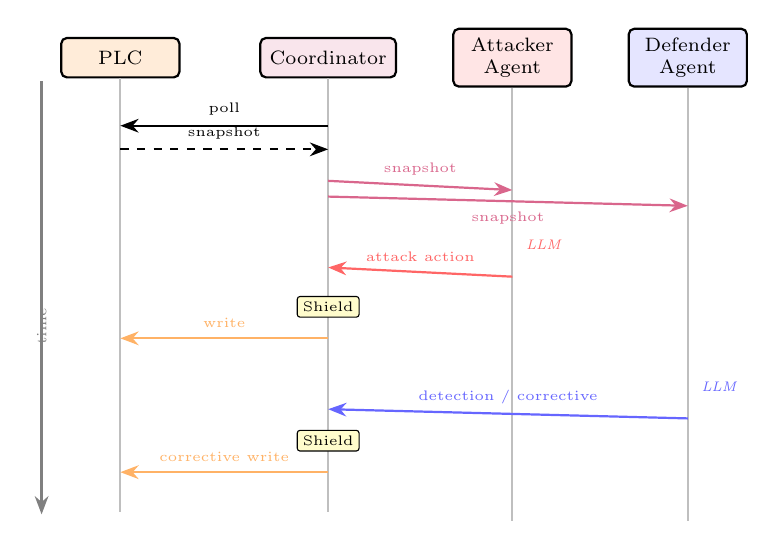
\begin{tikzpicture}[
        >=Stealth,
        node distance=0.4cm,
        every node/.style={font=\scriptsize},
        proc/.style={draw, rounded corners=2pt, minimum width=1.5cm, minimum height=0.5cm, align=center, thick},
        arr/.style={->, thick, >=Stealth},
    ]

    %% Participants
    \node[proc, fill=orange!15] (plc) {PLC};
    \node[proc, fill=purple!10, right=1.0cm of plc] (coord) {Coordinator};
    \node[proc, fill=red!10, right=0.7cm of coord] (atk) {Attacker\\Agent};
    \node[proc, fill=blue!10, right=0.7cm of atk] (def) {Defender\\Agent};

    %% Timeline
    \foreach \n in {plc, coord, atk, def} {
        \draw[thick, gray!50] (\n.south) -- ++(0,-5.5);
    }

    %% Step 1: Coordinator polls PLC
    \draw[arr] ([yshift=-0.6cm]coord.south) -- node[above, font=\tiny]{poll} ([yshift=-0.6cm]plc.south);
    \draw[arr, dashed] ([yshift=-0.9cm]plc.south) -- node[above, font=\tiny]{snapshot} ([yshift=-0.9cm]coord.south);

    %% Step 2: Broadcast to agents
    \draw[arr, purple!60] ([yshift=-1.3cm]coord.south) -- node[above, font=\tiny]{snapshot} ([yshift=-1.3cm]atk.south);
    \draw[arr, purple!60] ([yshift=-1.5cm]coord.south) -- node[below, font=\tiny]{snapshot} ([yshift=-1.5cm]def.south);

    %% Step 3: Attacker proposes attack
    \node[right=0.05cm, font=\tiny\itshape, text=red!60] at ([yshift=-2.0cm]atk.south) {LLM};
    \draw[arr, red!60] ([yshift=-2.4cm]atk.south) -- node[above, font=\tiny]{attack action} ([yshift=-2.4cm]coord.south);

    %% Step 4: Shield check
    \node[draw, fill=yellow!20, rounded corners=1pt, font=\tiny, inner sep=2pt] (sh) at ([yshift=-2.9cm, xshift=0cm]coord.south) {Shield};

    %% Step 5: Write to PLC
    \draw[arr, orange!60] ([yshift=-3.3cm]coord.south) -- node[above, font=\tiny]{write} ([yshift=-3.3cm]plc.south);

    %% Step 6: Defender detects
    \node[right=0.05cm, font=\tiny\itshape, text=blue!60] at ([yshift=-3.8cm]def.south) {LLM};
    \draw[arr, blue!60] ([yshift=-4.2cm]def.south) -- node[above, font=\tiny]{detection / corrective} ([yshift=-4.2cm]coord.south);

    %% Step 7: Shield + write corrective
    \node[draw, fill=yellow!20, rounded corners=1pt, font=\tiny, inner sep=2pt] at ([yshift=-4.6cm]coord.south) {Shield};
    \draw[arr, orange!60] ([yshift=-5.0cm]coord.south) -- node[above, font=\tiny]{corrective write} ([yshift=-5.0cm]plc.south);

    %% Time arrow
    \draw[arr, gray, thick] (-1.0, -0.3) -- (-1.0, -5.8) node[midway, left, font=\tiny, rotate=90]{time};

    \end{tikzpicture}
    \caption{Agent-mode interaction sequence. The coordinator mediates between the PLC, attacker agent, and defender agent. Both offensive and corrective writes pass through the safety shield.}
    \label{fig:agent-mode}
\end{figure}

\subsection{Design Principles}

The system design follows five principles:

\begin{itemize}[leftmargin=1.5em]
    \item \textbf{No unrestricted direct actuation from any LLM.} All writes are mediated by the safety shield.
    \item \textbf{All experiments are bounded by explicit safety rules.}
    \item \textbf{Every run produces replayable and auditable artifacts.}
    \item \textbf{The framework emphasises iterative attacker-defender interaction rather than one-shot evaluation.}
    \item \textbf{Agents are process-isolated and coordinator-mediated}, preventing any single component from monopolising PLC access.
\end{itemize}
\section{Implementation}
\label{sec:implementation}

This section describes the implementation of CPSForge. The system is built around a real Siemens S7 PLC connected to Factory~I/O (a software-based process emulator), with logic engineered in TIA Portal~v17. All experiments execute in a PLC-in-the-loop setting where the controller runs real scan cycles against emulated plant I/O.

\subsection{Hardware and Process Setup}

The controller layer consists of a Siemens S7-1200 PLC deployed with logic created in TIA Portal~v17. The PLC communicates over Ethernet at a fixed IP address (192.168.0.1). Factory~I/O serves as the process emulator, providing realistic industrial scenes with sensors, actuators, and stateful physical interaction. The PLC interacts with Factory~I/O through the normal control loop, while CPSForge observes and mediates selected control-relevant variables through an external middleware bridge implemented using the python-snap7 library~\cite{snap7}.

The current deployment supports five Factory~I/O scenes:

\begin{itemize}[leftmargin=1.5em]
    \item \textbf{From A to B:} a conveyor transport scene with 4 tags (conveyor, enable, state, item\_detected), exposing actuator override and sequence perturbation attack surfaces.
    \item \textbf{Filling Tank:} a discrete fill-cycle scene with 8 tags (fill pump, discharge pump, sensor, fill level, timers), exposing actuator override and setpoint shift attack surfaces.
    \item \textbf{Level Control:} a tank filling and draining scene with 15 tags (fill valve, discharge valve, liquid level, setpoints, enable), exposing setpoint shift and actuator override attack surfaces.
    \item \textbf{Sorting by Height:} a sorting conveyor scene with 30 tags (entry conveyor, transfer left/right, load/unload actuators, height sensors, enable), exposing a broader combinatorial attack surface.
    \item \textbf{Sorting by Weight:} a weight-threshold sorting scene with 35 tags (conveyor, weight sensor, threshold setpoints, pushers, reject lane), exposing setpoint shift attacks targeting classifier thresholds.
\end{itemize}

\subsection{Middleware Bridge}

A Python-based middleware layer communicates with the PLC via python-snap7, providing cyclic telemetry collection, action compilation, and structured logging. The middleware reads relevant tags at a configurable polling interval (default 500\,ms), constructs structured plant snapshots using Pydantic data models, and forwards context to the attacker and defender modules. Approved attack actions are translated into bounded PLC writes through the safety shield.

Each polling interval records: timestamp, scene identifier, sensor values, actuator states, controller mode bits, alarm status, setpoints, active attack context, shield decisions, and detector outputs. These records form the basis for both online monitoring and offline replay.

\subsection{Scene Profiles}

Each Factory~I/O scene is represented as a configurable YAML profile that defines tag metadata, process descriptions, writable variables exposed to the attacker, allowed attack types, safety invariants, reset behaviour, and sampling interval. This scene abstraction allows the core framework to remain independent of any one process while capturing scene-specific semantics.

\subsection{Attack Representation}

CPSForge does not permit attack modules to manipulate raw memory areas directly. Instead, the attacker outputs structured actions with fields such as target, mode, value, duration, rationale, and expected effect. This representation constrains the action space to meaningful process operations, enables validation by the shield, and makes experiments easier to replay and analyse.

\subsection{Campaign Attacker}

The campaign attacker extends the LLM batch attacker with a structured four-phase attack lifecycle: \emph{reconnaissance} (probing tag responses and process dynamics), \emph{preparation} (small perturbations to test detector sensitivity), \emph{exploitation} (targeted attacks informed by prior observations), and \emph{persistence} (sustained low-magnitude perturbations designed to remain undetected). Each phase is parameterised with a phase-specific objective prompt that receives the scene profile, current plant snapshot, action history with observed effects from prior phases, and phase-specific constraints. The LLM generates structured actions for each phase, and inter-phase delays allow the process to settle before the next phase begins. This design enables multi-step attack sequences where later phases exploit information gathered in earlier phases---for example, using reconnaissance observations to calibrate exploitation values just below detector thresholds.

\subsection{Safety Shield Implementation}

The shield is implemented as a policy enforcement layer with scene-specific rule support. Before a candidate action is executed, the shield checks whether the target is on the writable whitelist, whether the value falls within allowed bounds, whether the duration exceeds policy, and whether the action violates interlocks or state-based constraints. The shield emits a structured decision recording approval status, reasons, normalised values, violated rules, expiration times, and rollback procedures. Figure~\ref{fig:shield-flow} shows the decision flow.

In agent mode, the shield also validates defender corrective writes via \texttt{evaluate\_corrective()}, applying the same constraints used for attack actions.

\begin{figure}[t]
    \centering
    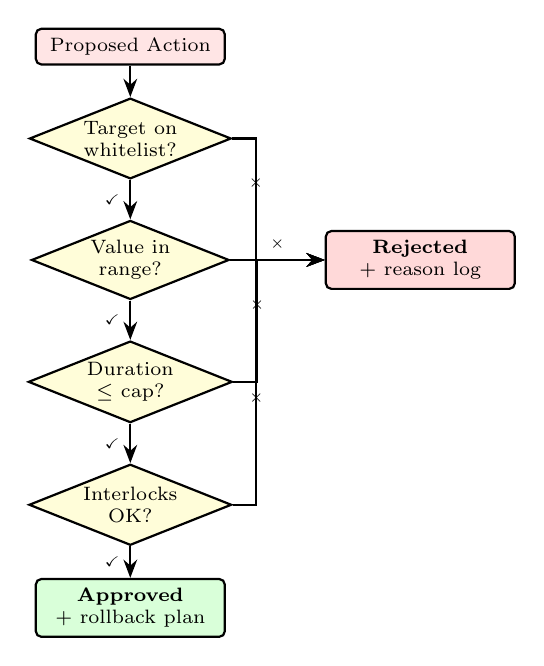
\begin{tikzpicture}[
        >=Stealth,
        node distance=0.3cm,
        every node/.style={font=\scriptsize},
        stepbox/.style={draw, rounded corners=2pt, minimum width=2.4cm, minimum height=0.45cm, align=center, thick},
        dec/.style={draw, diamond, aspect=2.5, inner sep=1pt, align=center, thick, font=\scriptsize},
        arr/.style={->, thick, >=Stealth},
    ]
    \node[stepbox, fill=red!10] (input) {Proposed Action};
    \node[dec, fill=yellow!15, below=0.4cm of input] (wl) {Target on\\whitelist?};
    \node[dec, fill=yellow!15, below=0.5cm of wl] (range) {Value in\\range?};
    \node[dec, fill=yellow!15, below=0.5cm of range] (dur) {Duration\\$\leq$ cap?};
    \node[dec, fill=yellow!15, below=0.5cm of dur] (interlock) {Interlocks\\OK?};
    \node[stepbox, fill=green!15, below=0.4cm of interlock] (approve) {\textbf{Approved}\\+ rollback plan};
    \node[stepbox, fill=red!15, right=1.2cm of range] (reject) {\textbf{Rejected}\\+ reason log};

    \draw[arr] (input) -- (wl);
    \draw[arr] (wl) -- node[left, font=\tiny]{\checkmark} (range);
    \draw[arr] (wl.east) -- ++(0.3,0) |- node[above, near start, font=\tiny]{$\times$} (reject);
    \draw[arr] (range) -- node[left, font=\tiny]{\checkmark} (dur);
    \draw[arr] (range.east) -- node[above, font=\tiny]{$\times$} (reject);
    \draw[arr] (dur) -- node[left, font=\tiny]{\checkmark} (interlock);
    \draw[arr] (dur.east) -- ++(0.3,0) |- node[above, near start, font=\tiny]{$\times$} (reject);
    \draw[arr] (interlock) -- node[left, font=\tiny]{\checkmark} (approve);
    \draw[arr] (interlock.east) -- ++(0.3,0) |- node[below, near start, font=\tiny]{$\times$} (reject);

    \end{tikzpicture}
    \caption{Safety shield decision flow. Each proposed action must pass four sequential checks before approval. Any failure produces a structured rejection with explicit reasons.}
    \label{fig:shield-flow}
\end{figure}

\subsection{Defender Stack}

The defender stack comprises six anomaly detection approaches spanning rule-based, statistical, and learned categories:

\begin{itemize}[leftmargin=1.5em]
    \item \textbf{Threshold detector:} configurable per-tag high/low bounds for simple process deviation detection.
    \item \textbf{Invariant detector:} rule-based checks derived from scene-specific safety invariants (e.g., actuator interlocks, mode-gated constraints).
    \item \textbf{CUSUM detector:} cumulative sum (CUSUM) change-point detection~\cite{page1954continuous} applied to each monitored tag, with configurable drift tolerance and decision threshold.
    \item \textbf{One-Class SVM (OCSVM):} a one-class support vector machine~\cite{scholkopf2001estimating} trained on normal-operation baseline traces, scoring each snapshot against the learned normal boundary.
    \item \textbf{Isolation Forest:} an unsupervised ensemble method~\cite{liu2008isolation} that isolates anomalies by random recursive partitioning of the feature space.
    \item \textbf{LSTM autoencoder (LSTM-AD):} a sequence-to-sequence LSTM autoencoder~\cite{malhotra2016lstm} trained to reconstruct sliding windows of normal process behaviour; anomalies are detected when reconstruction error exceeds a learned threshold.
\end{itemize}

The threshold and invariant detectors provide interpretable baselines requiring no training data. The ML-based detectors (OCSVM, Isolation Forest, LSTM-AD) are trained offline on baseline traces collected during normal plant operation and support both offline evaluation and online inference. All detectors implement a common interface supporting \texttt{observe}, \texttt{detect}, and \texttt{reset} operations.

\subsection{LLM Integration}
\label{sec:impl:llm}

CPSForge abstracts the LLM backend through a provider interface supporting OpenAI-compatible APIs, including local inference servers (e.g., LM Studio). The current deployment uses local models served at \texttt{http://127.0.0.1:1234/v1}: Qwen2-7B-Instruct for both batch-mode and agent-mode experiments. The provider includes an automatic system-role fallback that merges system prompts into user messages for models that do not support multi-role conversations.

The LLM integration layer includes:

\begin{itemize}[leftmargin=1.5em]
    \item \textbf{Prompt builder.} A versioned template system that constructs LLM prompts from scene profiles, plant snapshots, attacker/defender objectives, action history, and detection events. Templates are stored as text files and can be updated without code changes.
    \item \textbf{JSON schema validation.} LLM responses are parsed against attack and corrective-action schemas. A normalisation layer maps common key and attack-type aliases, unwraps nested JSON objects, and repairs malformed numeric fields. Invalid outputs trigger automatic retries with schema-correction prompts.
    \item \textbf{Safe parsing.} Responses are sanitised to prevent injection of raw PLC addresses or unsafe field values.
    \item \textbf{Run logging.} All prompts and responses are optionally logged with configurable redaction for reproducibility.
\end{itemize}

\subsection{Agent Mode Implementation}
\label{sec:impl:agent}

The agent mode uses Python's \texttt{multiprocessing} module to run the attacker and defender as independent OS processes. Each agent communicates with the coordinator through typed \texttt{multiprocessing.Queue} channels. The coordinator runs the PLC polling loop and dispatches actions:

\begin{enumerate}[leftmargin=1.5em]
    \item The coordinator polls PLC tags and broadcasts a plant snapshot to both agents.
    \item The attacker agent invokes its LLM with scene context, snapshot, and action history, producing an attack action.
    \item The coordinator validates the action through the safety shield, executes approved writes, and logs the result.
    \item The defender agent receives the same snapshot (and optionally the attacker's action after execution), invokes its LLM to diagnose process state, and may propose a corrective write.
    \item Corrective writes pass through the same shield before execution.
\end{enumerate}

The coordinator enforces per-agent timeouts, graceful shutdown on errors, and configurable cooldown between actions. All agent messages and decisions are logged as structured artifacts for post-hoc analysis.

\subsection{Closed-Loop Data Management}

Every experiment run produces structured artifacts for replay and analysis. A run folder contains the time-series trace, metadata, attack records, shield decisions, and detection outputs. Runs that lead to missed or delayed detections are marked as hard cases and placed into a replay bank for future defender refinement.

The pipeline is fully operational: evaluation runs have been executed against the real PLC across five Factory~I/O scenes using scripted, random, LLM batch, campaign, and LLM agent attackers, and a closed-loop adaptation protocol has been validated across two scenes with both rule-based and campaign attackers. Results are presented in Section~\ref{sec:evaluation}.
\section{Methodology}
\label{sec:methodology}

Our evaluation methodology measures attacker effectiveness, shield safety, defender robustness, and adaptation gains in a closed-loop CPS setting. Figure~\ref{fig:pipeline} illustrates the experiment pipeline from action generation through execution and detection.

\begin{figure}[t]
    \centering
    \begin{tikzpicture}[
        >=Stealth,
        node distance=0.35cm,
        every node/.style={font=\scriptsize},
        step/.style={draw, rounded corners=2pt, minimum width=2.8cm, minimum height=0.5cm, align=center, thick},
        decision/.style={draw, diamond, aspect=2.2, minimum width=1.5cm, inner sep=1pt, align=center, thick},
        arr/.style={->, thick, >=Stealth},
    ]

    %% Pipeline steps
    \node[step, fill=gray!10] (init) {1. Initialise PLC \&\\Factory~I/O scene};
    \node[step, fill=gray!10, below=of init] (warmup) {2. Warm-up period\\(baseline telemetry)};
    \node[step, fill=red!10, below=of warmup] (propose) {3. Attacker proposes\\structured action(s)};
    \node[step, fill=yellow!15, below=of propose] (validate) {4. JSON schema\\validation \& normalise};
    \node[decision, fill=yellow!20, below=0.45cm of validate] (shield) {Shield\\check?};
    \node[step, fill=green!10, below left=0.5cm and -0.3cm of shield] (exec) {5. Execute on\\live PLC};
    \node[step, fill=red!5, below right=0.5cm and -0.3cm of shield] (reject) {Reject \&\\log reason};
    \node[step, fill=blue!10, below=0.8cm of shield] (detect) {6. Defenders\\observe \& score};
    \node[decision, fill=blue!15, below=0.45cm of detect] (detected) {Attack\\detected?};
    \node[step, fill=green!10, below left=0.45cm and -0.3cm of detected] (alert) {Emit\\alert};
    \node[step, fill=orange!10, below right=0.45cm and -0.3cm of detected] (hardcase) {Hard case\\$\to$ bank};
    \node[step, fill=gray!10, below=0.8cm of detected] (log) {7. Record artifacts\\(Parquet, JSON)};

    %% Arrows
    \draw[arr] (init) -- (warmup);
    \draw[arr] (warmup) -- (propose);
    \draw[arr] (propose) -- (validate);
    \draw[arr] (validate) -- (shield);
    \draw[arr] (shield) -- node[left, font=\tiny]{\checkmark} (exec);
    \draw[arr] (shield) -- node[right, font=\tiny]{$\times$} (reject);
    \draw[arr] (exec) |- (detect);
    \draw[arr] (detect) -- (detected);
    \draw[arr] (detected) -- node[left, font=\tiny]{yes} (alert);
    \draw[arr] (detected) -- node[right, font=\tiny]{no} (hardcase);
    \draw[arr] (alert) |- (log);
    \draw[arr] (hardcase) |- (log);

    \end{tikzpicture}
    \caption{Batch-mode experiment pipeline. Each proposed action passes through schema validation and the safety shield before PLC execution. Undetected attacks are stored as hard cases for adaptation.}
    \label{fig:pipeline}
\end{figure}

\subsection{Experiment Workflow}
Each experiment proceeds as follows:
\begin{enumerate}[leftmargin=1.2em]
    \item Initialise the process in a known safe state.
    \item Start the PLC--Factory~I/O control loop and the logging service.
    \item Execute a benign warm-up period to establish baseline telemetry.
    \item Invoke the attacker to propose one or more structured actions.
    \item Pass each action through the safety shield.
    \item Execute approved actions and continue polling.
    \item Run defenders online over the collected snapshots.
    \item Record attack outcome, physical impact, detector behaviour, and shield events.
    \item Store the run as a replayable artifact.
\end{enumerate}

In agent mode, steps 4--7 are replaced by continuous concurrent operation: the attacker and defender agents independently observe plant state and propose actions, all mediated by the coordinator.

\subsection{Attacker Variants}
We compare four attacker classes:
\begin{itemize}[leftmargin=1.2em]
    \item \textbf{Scripted attacker:} deterministic templates with targeted process-aware actions.
    \item \textbf{Random attacker:} bounded random perturbations over the configured attack surface.
    \item \textbf{LLM attacker (batch):} process-aware planning over structured scene and state context, executed through the batch orchestration pipeline.
    \item \textbf{LLM attacker agent:} an autonomous LLM agent that observes plant state in real time, maintains action history with feedback, and proposes attacks concurrently with the defender agent.
\end{itemize}

\subsection{Defender Variants}
We evaluate four defender configurations:
\begin{itemize}[leftmargin=1.2em]
    \item \textbf{Threshold detector:} configurable per-tag thresholds with severity levels.
    \item \textbf{Invariant detector:} rule-based state-consistency checks derived from scene-specific safety properties.
    \item \textbf{Sequence detector:} a sliding-window ML model for temporal anomaly detection.
    \item \textbf{LLM defender agent:} an autonomous LLM agent (agent mode only) that analyses process telemetry, diagnoses anomalies, and proposes corrective actions.
\end{itemize}

\subsection{Metrics}
We measure:
\begin{itemize}[leftmargin=1.2em]
    \item \textbf{Attack validity:} fraction of attacker outputs that compile and execute successfully.
    \item \textbf{Attack success:} fraction of attacks that produce measurable process deviation.
    \item \textbf{Physical impact:} process deviation measured as the difference between attack-period and baseline tag values.
    \item \textbf{Shield effectiveness:} fraction of proposals approved versus rejected, and unsafe action block rate.
    \item \textbf{Detection performance:} precision, recall, F1, false-positive count, and detection latency.
    \item \textbf{Adaptation gain:} improvement in detection robustness across iterative rounds.
\end{itemize}

For agent mode experiments, we additionally report:
\begin{itemize}[leftmargin=1.2em]
    \item \textbf{Agent actions per round:} number of attack and corrective actions proposed per run.
    \item \textbf{Corrective success rate:} fraction of defender corrective actions that restore process state.
    \item \textbf{Adversarial dynamics:} temporal interplay between attacker perturbations and defender corrections.
\end{itemize}

\subsection{Scenes and Scale}

The evaluation covers three Factory~I/O scenes of increasing complexity: From A to B (4 tags, discrete transport), Level Control (15 tags, continuous process), and Sorting by Height (30 tags, mixed discrete/continuous). For batch mode, each attacker variant is evaluated per scene. For agent mode, LLM attacker and LLM defender agents are evaluated on each scene. Each configuration runs 120--200 steps at a 500\,ms polling interval against the live PLC.

\subsection{Closed-Loop Adaptation}
After each evaluation round, traces corresponding to missed or weakly detected attacks are added to a hard-case bank. These traces are used to refine learned defenders or detector policies in the next round. We measure adaptation gain as the improvement in detection F1 between the initial round and subsequent rounds trained on accumulated hard cases.

\subsection{Ground Truth}
\label{sec:methodology:gt}
Ground-truth labelling is derived from the experiment protocol itself. Each polling step is labelled as \emph{attack-active} or \emph{normal} based on whether a shield-approved attack action was active during that step. This label is recorded in the trace metadata at runtime, not post hoc. Baseline normal-operation traces (no attacker active) are collected for each scene to provide unlabelled ground truth for anomaly-detection calibration.
\section{Evaluation}
\label{sec:evaluation}

This section evaluates CPSForge as a closed-loop LLM red/blue team framework across three Factory~I/O scenes on a real Siemens S7-1200 PLC. All reported numbers are collected from live PLC runs; no results are simulated or mocked.

\subsection{Research Questions}

\begin{description}[leftmargin=1.5em, style=nextline]
    \item[RQ1 (Context Ablation):] How does operational context (minimal vs.\ partial vs.\ full) affect the capability of a local LLM to launch successful CPS attacks?
    \item[RQ2 (Fine-Tuning):] How does task-specific QLoRA fine-tuning change attack capability, stealth, validity, and cross-scene transfer on Qwen2.5-3B-Instruct?
    \item[RQ3 (Attack Mode):] Can an online MITM LLM attacker exploit timing and phase transitions more effectively than a static one-shot LLM or a random baseline?
    \item[RQ4 (Defenses):] Which runtime defenses remain effective against context-aware, timing-aware LLM attackers? Does an LLM defender outperform rule-based defenses?
    \item[RQ5 (Cross-Model Robustness):] Are the observed attack and defense trends robust across three local models from two families, or are they strongly model-specific?
    \item[RQ6 (Frontier Model):] Does a frontier API model (GPT-4o-mini) exhibit qualitatively different attack capability, self-deterrence behavior, or defense evasion compared to local 3B-class models?
\end{description}

\subsection{Evaluation Environment}

Experiments are conducted on a real Siemens S7-1200 PLC connected to Factory~I/O~\cite{factoryio} through TIA Portal~v17~\cite{tiaportal}. The evaluation covers three scenes: Level Control (continuous tank process, 15~tags), Sorting by Height (discrete 2-way height sorting, 30~tags), and Sorting by Weight (discrete 3-way weight sorting, 35~tags). The middleware polls PLC tags at 500\,ms intervals via python-snap7~\cite{snap7}; the LLM attacker is called every three polling cycles. We note that the S7-1200 PLC scan cycle is typically 1--10\,ms; the 500\,ms polling interval is a middleware-level parameter that determines observation granularity, not PLC control speed. Attack effects that occur and are corrected within a single polling interval may not be observable.

All LLM inference runs in-process via HuggingFace \texttt{transformers} with 4-bit NF4 quantization through \texttt{bitsandbytes}. No external inference server is used. The primary model is Qwen2.5-3B-Instruct (${\sim}$6\,GB), studied in base form. Two additional cross-model comparison models are used for RQ5: Qwen3-1.7B (${\sim}$4\,GB) and SmolLM3-3B (${\sim}$6\,GB). Experiments run on a Dell Precision 5820 with an NVIDIA RTX A4000 (16\,GB VRAM) under Windows~11 Enterprise.

The completed experiment matrix comprises 333~runs: 27~(RQ1) + 36~(RQ2) + 27~(RQ3) + 126~(RQ4, base + finetuned) + 72~(RQ5) + 45~(RQ6). Each run executes 60~steps at 500\,ms polling (30\,s of PLC polling time). Including LLM inference---13--33\,s per call at up to 20~calls per run for local models, 2--5\,s for the API model---total wall-clock time is approximately 1--10~minutes per run. Each run produces a unified per-step log (Parquet with 33+ fields), attack records, shield decisions, PLC event captures, and summary metrics (all JSON).

\subsection{Attacker Configurations}

We compare three attacker modes (RQ3), each producing the same unified per-step log format:

\begin{itemize}[leftmargin=1.5em]
    \item \textbf{Random baseline:} bounded random perturbations over the configured attack surface, providing a lower bound on attacker capability. Always attacks (no wait decisions).
    \item \textbf{Static LLM:} a one-shot batch attacker that receives full context once and generates attack proposals without observing process feedback. Tests LLM attack capability without online adaptation.
    \item \textbf{Online MITM:} the core contribution (C1). An iterative observe--decide--act loop where the LLM observes live plant state every three control cycles, infers the current process phase, builds a context-tier-specific prompt, and decides to \emph{attack} or \emph{wait}. All writes pass through the full defense chain before reaching the PLC.
\end{itemize}

\subsection{Defense Configurations}

We evaluate seven defense variants for RQ4:

\begin{itemize}[leftmargin=1.5em]
    \item \textbf{None:} no defense (measures raw attacker capability).
    \item \textbf{Baseline:} threshold and invariant detectors.
    \item \textbf{Phase-aware shield (C4):} blocks writes inconsistent with the inferred process phase.
    \item \textbf{Intent-consistency checker (C4):} blocks writes opposing the controller's current trend.
    \item \textbf{Combined:} phase-aware shield + intent-consistency checker together.
    \item \textbf{LLM defender (novel):} an LLM-based anomaly scorer using the same model and context pipeline as the attacker. Evaluates each proposed write and decides allow/block with a suspicion score.
    \item \textbf{LLM combined:} phase-aware + intent-consistency + LLM defender together.
\end{itemize}

\subsection{Metrics}

\textbf{Attacker metrics.} Attack Success Rate (ASR) $= N_{\text{succ}}/N_{\text{exec}}$, computed post-hoc: for write at step $N$, compare tag value at step $N{-}1$ vs.\ $N{+}2$; success if the tag moved toward the injected value. Valid Action Rate (VAR) $= N_{\text{schema\_valid}}/N_{\text{submitted}}$, and mean LLM inference latency (ms).

\textbf{Defense metrics.} Prevention rate $= N_{\text{blocked}}/N_{\text{proposals}}$, measuring the fraction of attack proposals blocked before PLC write. Includes safety-shield blocks; rows where ``None'' defense shows nonzero prevention reflect mandatory safety-shield blocking, not RQ4 defense activation. Per-stage block counts (Ph., Int., LLM columns) identify the specific defense stage that blocked each proposal.

\textbf{Statistical note.} All tables report 3-repeat cells. For rare-event metrics (ASR), point estimates carry wide uncertainty (95\% CI width $\approx \pm 30\,\text{pp}$ for $n \leq 10$ writes). Findings are supported where multiple independent cells show the same pattern.

\subsection{Results}

\textbf{Safety-shield caveat.} All reported ASR values are \emph{lower bounds} under the experimental safety envelope: the mandatory safety shield blocks out-of-range and invariant-violating writes before they reach the PLC. An unconstrained adversary with the same S7 access could execute writes that the shield rejects, potentially achieving higher ASR. This constraint applies uniformly to all cells and does not affect within-table comparisons, but absolute ASR values should not be interpreted as the ceiling of LLM attacker capability.

\subsubsection{RQ1: Context Ablation}
\label{sec:eval:rq1}

Table~\ref{tab:context_ablation} shows the effect of operational context on attack capability using Qwen2.5-3B-Instruct (base) as the online MITM attacker with no defense active.

% Table 3 --- RQ1 Context Ablation
% Generated by: python -m cpsforge.analysis.generate_tables
% RQ-specific filtering: limited to 3 runs per (scene, context) cell
\begin{table}[t]
\centering
\caption{RQ1: Context ablation for online MITM attacker (base Qwen2.5-3B; no RQ4 defense active; safety shield always active).}
\label{tab:context_ablation}
\small
\setlength{\tabcolsep}{3pt}
\begin{tabular}{llrrrrrr}
\toprule
\textbf{Scene} & \textbf{Context} & \textbf{Runs} & \textbf{Prop.} & \textbf{Writes} & \textbf{Succ.} & \textbf{ASR\%} & \textbf{Lat.(ms)} \\
\midrule
Level Control & Minimal & 3 & 23 & 2 & 0 & 0.0 & 13086 \\
 & Partial & 3 & 20 & 13 & 0 & 0.0 & 18429 \\
 & Full & 3 & 5 & 0 & 0 & 0.0 & 7863 \\
\midrule
Sort.~Weight & Minimal & 3 & 13 & 13 & 7 & 53.8 & 17929 \\
 & Partial & 3 & 12 & 5 & 2 & 40.0 & 19789 \\
 & Full & 3 & 0 & 0 & 0 & 0.0 & 11180 \\
\midrule
Sort.~Height & Minimal & 3 & 30 & 30 & 1 & 3.3 & 16906 \\
 & Partial & 3 & 30 & 25 & 1 & 4.0 & 22944 \\
 & Full & 3 & 30 & 30 & 4 & 13.3 & 22263 \\
\bottomrule
\end{tabular}
\vspace{2pt}
\noindent\footnotesize{3 repeats per configuration; ASR computed post-hoc.}
\end{table}

\textbf{Finding 1: Full context causes self-deterrence on Sorting by Weight and near-complete suppression on Level Control.} Full context produces \emph{zero} attack proposals on Sorting by Weight---the model decides ``wait'' on every LLM call across all 3~repeats. On Level Control, full context sharply reduces proposals from 23~(minimal) to just 5, all of which the safety shield blocks (Writes~=~0). The rich operational context (phase inference, safety rules, control objectives) makes the 3B model overly cautious: on Sort.~Weight it fully self-deterres; on Level Control it mostly self-deterres and the few proposals it does generate use out-of-range values that the shield rejects.

\textbf{Finding 2: Self-deterrence is scene-dependent.} On Sorting by Weight, partial context achieves 40.0\% ASR vs.\ 53.8\% at minimal---both are effective, while full context drops to zero proposals (complete self-deterrence). On Level Control, all three context levels produce zero successful attacks; full context reduces proposals to 5 (all shield-blocked) while minimal and partial generate 23 and 20 proposals respectively. On Sorting by Height, full context is the \emph{most} effective tier (13.3\% ASR vs.\ 3.3\% and 4.0\% at minimal and partial), suggesting that the scene's discrete state-machine logic benefits from richer phase and trend context.

\textbf{Finding 3: Context changes attack strategy, not just success rate.} With minimal context, the model uses brute-force actuator overrides. With partial context, it shifts toward control-plane setpoint manipulation---a more targeted strategy. Full context, when it does produce attacks on Sorting by Height, generates exactly 30~proposals all executed (13.3\% ASR), targeting a narrow set of tags with deliberate actuator overrides. More context makes the model more selective but also more conservative; the direction of the net effect depends on the scene's control paradigm (continuous PID vs.\ discrete state machine).

\textbf{Note on Level Control results.} Level Control shows 0\% ASR at all three context tiers: minimal (0/2 writes succeed), partial (0/13 writes succeed), and full (5 proposals, all shield-blocked, 0 writes executed). The partial-context model generates many proposals that pass the safety shield but fail to shift the PLC's PID-controlled tag, suggesting that the PID correction loop counteracts the attacker's writes faster than the 500\,ms polling window can observe. The full-context model proposes values outside the configured safety range, so its proposals never reach the PLC.

\textbf{Implication for defense:} The self-deterrence effect suggests that \emph{exposing operational context may itself be a defense mechanism}---a form of deterrence through transparency that reduces LLM red team effectiveness without any active blocking.

\subsubsection{RQ2: Fine-Tuning Impact}
\label{sec:eval:rq2}

RQ2 measures how task-specific QLoRA fine-tuning changes \emph{both} red team (attack) and blue team (defense) capability on the same model. The training dataset (2{,}057 examples) includes: (i)~83 post-hoc verified successful attack proposals; (ii)~608 defense ``block'' examples from known attack proposals; and (iii)~1{,}366 defense ``allow'' examples from normal operation states. Fine-tuning uses QLoRA (rank=16, $\alpha$=32) on Qwen2.5-3B-Instruct in 4-bit NF4 quantization for 3~epochs.

\textbf{Training procedure.} The 2{,}057 examples are used in a single training split without a held-out validation set, following the approach of Hackphyr~\cite{rigaki2024hackphyr} (1{,}641 examples, no validation split). We monitor training loss, which decreases monotonically from 1.82 to 0.41 over 3~epochs. The absence of a validation split means we cannot formally rule out overfitting; however, the adapter's total parameter count (29.9M, 0.96\% of the 3.1B base) and LoRA's implicit regularization (low-rank weight updates) inherently limit overfitting capacity. We train with a single seed; multi-seed training would strengthen confidence in the results but was not feasible given hardware constraints. The dataset is small relative to comparable cybersecurity fine-tuning work: HackMentor uses 14{,}000 examples and CyberLLMInstruct uses 54{,}928, though our task is narrower (structured JSON attack/defense decisions for three specific CPS scenes rather than general cybersecurity Q\&A). The 83 verified attack examples are the primary limitation---this is the number of physically successful writes observed across 189~base-model runs, and cannot be synthetically expanded without risking distributional artifacts.

Table~\ref{tab:finetune_comparison} shows the results.

% Table RQ2 --- Fine-Tuning Comparison
% Generated by: python -m cpsforge.analysis.generate_tables
% RQ-specific filtering: limited to 3 runs per (scene, context, model) cell
\begin{table}[t]
\centering
\caption{RQ2: Fine-tuning effect on attack capability (online MITM, no defense). Base = Qwen2.5-3B-Instruct; FT = same model with QLoRA v2 adapter. VAR = schema-valid outputs / LLM calls.}
\label{tab:finetune_comparison}
\small
\setlength{\tabcolsep}{3pt}
\resizebox{\columnwidth}{!}{%
\begin{tabular}{lllrrrrrrr}
\toprule
\textbf{Scene} & \textbf{Ctx} & \textbf{Model} & \textbf{Runs} & \textbf{LLM calls} & \textbf{VAR\%} & \textbf{Prop.} & \textbf{Writes} & \textbf{Succ.} & \textbf{ASR\%} \\
\midrule
Level Control & Minimal & Base & 3 & 27 & 100.0 & 23 & 2 & 0 & 0.0 \\
 & Minimal & FT & 3 & 30 & 100.0 & 30 & 30 & 11 & 36.7 \\
 & Full & Base & 3 & 15 & 100.0 & 5 & 0 & 0 & 0.0 \\
 & Full & FT & 3 & 34 & 0.0 & 0 & 0 & 0 & 0.0 \\
\midrule
Sort.~Weight & Minimal & Base & 3 & 14 & 92.9 & 13 & 13 & 7 & 53.8 \\
 & Minimal & FT & 3 & 30 & 100.0 & 30 & 16 & 0 & 0.0 \\
 & Full & Base & 3 & 5 & 40.0 & 0 & 0 & 0 & 0.0 \\
 & Full & FT & 3 & 60 & 0.0 & 0 & 0 & 0 & 0.0 \\
\midrule
Sort.~Height & Minimal & Base & 3 & 30 & 100.0 & 30 & 30 & 1 & 3.3 \\
 & Minimal & FT & 3 & 30 & 100.0 & 30 & 30 & 3 & 10.0 \\
 & Full & Base & 3 & 30 & 100.0 & 30 & 30 & 4 & 13.3 \\
 & Full & FT & 3 & 45 & 0.0 & 0 & 0 & 0 & 0.0 \\
\bottomrule
\end{tabular}%
}
\vspace{2pt}
\noindent\footnotesize{3 repeats per configuration; ASR computed post-hoc.}
\end{table}

\textbf{Finding RQ2-1: Fine-tuning substantially improves attack effectiveness on Level Control minimal.} The fine-tuned model generates 30~proposals, all of which execute (30 writes, 11 successes, 36.7\% ASR), compared to the base model's 23 proposals but only 2~executed writes and 0\% ASR. Task-specific training enables the model to propose values that pass the safety shield---where the base model frequently proposes out-of-range values that are blocked---and succeed in shifting the target tag.

\textbf{Finding RQ2-2: Fine-tuning does not improve all scenes uniformly.} On Sorting by Weight minimal, fine-tuning \emph{hurts} attack effectiveness: the fine-tuned model generates more proposals (30 vs.\ 13) but achieves 0\% ASR compared to 53.8\% for the base. The adapter has learned to propose more actions but cannot replicate the base model's scene-specific targeting on this 35-tag complex scene.

\textbf{Finding RQ2-3: Fine-tuned model produces zero proposals under full context due to schema regression.} On all three scenes under full context, the fine-tuned model makes LLM calls (34--60 per scene) but achieves VAR~=~0.0\%---every output fails schema validation. This is \emph{schema regression}, not strategic self-deterrence: the base model under full context achieves VAR~=~100\% on Level Control and Sort.~Height (issuing valid ``wait'' decisions) and VAR~=~40\% on Sort.~Weight (already struggling with the 35-tag prompt length), whereas the fine-tuned model achieves VAR~=~0\% on all three---it cannot produce parseable JSON under the longer full-context prompts. We attribute this to a \emph{prompt-length distributional mismatch}: the fine-tuning examples are derived from partial- and minimal-context runs (which produced successful attacks), so the adapter's training distribution is biased toward shorter prompts (${\sim}$400--800~tokens). Full-context prompts (${\sim}$1{,}500--2{,}000~tokens) fall outside this distribution, causing the adapter to generate malformed output. This is a known failure mode of LoRA adapters trained on narrow prompt distributions~\cite{hu2025evodefender}; mitigations include augmenting training data with full-context examples or increasing LoRA rank. Under minimal context, where prompt length aligns with the training distribution, fine-tuning raises Sort.~Height ASR from 3.3\% to 10.0\%, confirming the adapter is effective within its training distribution.

\textbf{Mitigation note.} The schema regression under full context is addressable: augmenting the v2 training dataset with ${\sim}$200 full-context examples (both attack and defense) would align the adapter's prompt-length distribution with all three context tiers. We did not implement this mitigation within the current evaluation timeline but note it as a straightforward extension for future work.

\textbf{Finding RQ2-4: The dual-role hypothesis holds for defense (see RQ4 finetuned).} Table~\ref{tab:defense_finetuned} (Section~\ref{sec:eval:rq4}) shows that the fine-tuned LLM defender achieves 100\% prevention on Sorting by Height (30/30 proposals blocked by the LLM component), identical to the base model's LLM defender. Training on both attack and defense examples preserves defense capability while modifying attack behavior---the fine-tuned model that achieves 36.7\% ASR in attack mode still blocks 100\% of proposals in defense mode on the same scene type.

\subsubsection{RQ3: Online vs.\ Static Attack Mode}
\label{sec:eval:rq3}

Table~\ref{tab:attacker_comparison} compares the three attacker modes across all three scenes with no defense active.

% Table 4 --- RQ3 Attacker Comparison
% Generated by: python -m cpsforge.analysis.generate_tables
% RQ-specific filtering: limited to 3 runs per (scene, attacker) cell
\begin{table}[t]
\centering
\caption{RQ3: Attacker comparison (base Qwen2.5-3B, no defense). Random = bounded random perturbations; Static LLM = one-shot batch; Online MITM = core contribution.}
\label{tab:attacker_comparison}
\small
\setlength{\tabcolsep}{3pt}
\begin{tabular}{llrrrrr}
\toprule
\textbf{Scene} & \textbf{Attacker} & \textbf{Runs} & \textbf{Prop.} & \textbf{Writes} & \textbf{Succ.} & \textbf{ASR\%} \\
\midrule
Level Control & Random & 3 & 10 & 10 & 1 & 10.0 \\
 & Static LLM & 3 & 0 & 0 & 0 & 0.0 \\
 & Online MITM & 3 & 14 & 0 & 0 & 0.0 \\
\midrule
Sort.~Weight & Random & 3 & 0 & 0 & 0 & 0.0 \\
 & Static LLM & 3 & 0 & 0 & 0 & 0.0 \\
 & Online MITM & 3 & 13 & 13 & 7 & 53.8 \\
\midrule
Sort.~Height & Random & 3 & 30 & 30 & 4 & 13.3 \\
 & Static LLM & 3 & 0 & 0 & 0 & 0.0 \\
 & Online MITM & 3 & 30 & 30 & 1 & 3.3 \\
\bottomrule
\end{tabular}
\vspace{2pt}
\noindent\footnotesize{3 repeats per configuration; ASR computed post-hoc.}
\end{table}

\textbf{Finding 4: Static LLM generates zero valid proposals under the batch design.} The static one-shot LLM produces no schema-valid attack proposals across all scenes. The batch attacker requests a full JSON array of up to 10 attack objects in a single call with a 350-token output budget---insufficient for the full array. Even after truncation repair (salvaging any complete objects from a partial response), zero schema-valid proposals survive. This reflects two concurrent constraints: (i)~the 350-token limit is too small for a multi-object JSON array, and (ii)~without iterative plant feedback, the model produces low-confidence generic outputs that fail schema validation. \textbf{Important caveat:} the 0\% result reflects our specific experimental design (350-token budget, batch JSON array format) rather than a fundamental limitation of one-shot LLM attack capability. AttackLLM~\cite{ahmed2025attackllm} uses GPT-4 with much larger context and output windows plus human-in-the-loop validation; such a design would likely overcome the token-budget constraint. We report the static result as evidence that \emph{our} batch design is ineffective, not that all one-shot designs are inherently incapable. The random baseline, which operates without any LLM call, achieves 10.0\% on Level Control and 13.3\% on Sorting by Height, establishing that the 0\% static LLM result is not the floor for all non-online approaches.

\textbf{Finding 5: Online MITM is the only effective attacker on complex scenes.} On Sorting by Weight, the online MITM achieves 53.8\% ASR while both random and static attackers generate zero proposals. The LLM's ability to reason about the 35-tag scene's control logic and select appropriate targets is essential---random perturbations cannot identify valid attack surfaces on complex scenes.

\textbf{Finding 6: Random baseline is competitive on discrete scenes.} On Sorting by Height, the random baseline achieves 13.3\% ASR compared to 3.3\% for the online MITM (3 runs each). Discrete sorting scenes have binary actuators where random single-tag overrides can accidentally align with vulnerable states, while the LLM's cautious wait/attack reasoning sometimes misses opportunistic windows.

\textbf{Finding 7: Level Control is resistant to all attacker types.} On Level Control, random achieves 10.0\% ASR with 10 writes, and static LLM generates 0 proposals. The online MITM generates 14 proposals but all are blocked by the safety shield (Writes~=~0)---the LLM proposes out-of-range values that fail the shield's range check, so no writes reach the PLC. This differs from the RQ1 partial-context result (Table~\ref{tab:context_ablation}), where 13~writes \emph{do} execute but 0 succeed: there, the PID correction loop counteracts valid writes faster than the polling window observes. Level Control's resilience thus has two layers: the safety shield blocks out-of-range proposals, and the PID controller corrects in-range writes.

\subsubsection{RQ4: Defense Effectiveness}
\label{sec:eval:rq4}

Table~\ref{tab:defense_comparison} presents the defense comparison across all three scenes using the base Qwen2.5-3B-Instruct model.

% Table 5 --- RQ4 Defense Comparison
% Generated by: python -m cpsforge.analysis.generate_tables
% RQ-specific filtering: limited to 3 runs per (scene, defense) cell
\begin{table}[t]
\centering
\caption{RQ4: Defense comparison for online MITM attacker (base Qwen2.5-3B). Prevention rate = fraction of attack proposals blocked before PLC write. ``None'' = no RQ4 defense; the mandatory safety shield (always active) accounts for any nonzero Blk.\ in ``None'' rows.}
\label{tab:defense_comparison}
\small
\setlength{\tabcolsep}{2pt}
\resizebox{\columnwidth}{!}{%
\begin{tabular}{llrrrrrrrrrr}
\toprule
\textbf{Scene} & \textbf{Defense} & \textbf{Runs} & \textbf{Prop.} & \textbf{Blk.} & \textbf{Wr.} & \textbf{Succ.} & \textbf{ASR\%} & \textbf{Prev.\%} & \textbf{Ph.} & \textbf{Int.} & \textbf{LLM} \\
\midrule
Level Control & None & 3 & 14 & 14 & 0 & 0 & 0.0 & 100.0 & 0 & 0 & 0 \\
 & Baseline & 3 & 0 & 0 & 0 & 0 & 0.0 & 0.0 & 0 & 0 & 0 \\
 & Phase-Aware & 3 & 0 & 0 & 0 & 0 & 0.0 & 0.0 & 0 & 0 & 0 \\
 & Intent & 3 & 18 & 0 & 18 & 3 & 16.7 & 0.0 & 0 & 0 & 0 \\
 & Combined & 3 & 0 & 0 & 0 & 0 & 0.0 & 0.0 & 0 & 0 & 0 \\
 & LLM Defender & 3 & 0 & 0 & 0 & 0 & 0.0 & 0.0 & 0 & 0 & 0 \\
 & LLM+Combined & 3 & 0 & 0 & 0 & 0 & 0.0 & 0.0 & 0 & 0 & 0 \\
\midrule
Sort.~Weight & None & 3 & 13 & 0 & 13 & 7 & 53.8 & 0.0 & 0 & 0 & 0 \\
 & Baseline & 3 & 0 & 0 & 0 & 0 & 0.0 & 0.0 & 0 & 0 & 0 \\
 & Phase-Aware & 3 & 0 & 0 & 0 & 0 & 0.0 & 0.0 & 0 & 0 & 0 \\
 & Intent & 3 & 0 & 0 & 0 & 0 & 0.0 & 0.0 & 0 & 0 & 0 \\
 & Combined & 3 & 0 & 0 & 0 & 0 & 0.0 & 0.0 & 0 & 0 & 0 \\
 & LLM Defender & 3 & 0 & 0 & 0 & 0 & 0.0 & 0.0 & 0 & 0 & 0 \\
 & LLM+Combined & 3 & 0 & 0 & 0 & 0 & 0.0 & 0.0 & 0 & 0 & 0 \\
\midrule
Sort.~Height & None & 3 & 30 & 0 & 30 & 1 & 3.3 & 0.0 & 0 & 0 & 0 \\
 & Baseline & 3 & 30 & 0 & 30 & 4 & 13.3 & 0.0 & 0 & 0 & 0 \\
 & Phase-Aware & 3 & 28 & 0 & 28 & 0 & 0.0 & 0.0 & 0 & 0 & 0 \\
 & Intent & 3 & 27 & 0 & 27 & 2 & 7.4 & 0.0 & 0 & 0 & 0 \\
 & Combined & 3 & 30 & 0 & 30 & 5 & 16.7 & 0.0 & 0 & 0 & 0 \\
 & LLM Defender & 3 & 30 & 30 & 0 & 0 & 0.0 & 100.0 & 0 & 0 & 30 \\
 & LLM+Combined & 3 & 28 & 28 & 0 & 0 & 0.0 & 100.0 & 0 & 0 & 28 \\
\bottomrule
\end{tabular}%
}
\vspace{2pt}
\noindent\footnotesize{3 repeats per configuration; ASR computed post-hoc.}
\end{table}

\textbf{Finding 8: The LLM defender achieves 100\% prevention on Sorting by Height.} The LLM-based anomaly defender blocked all 30 attack proposals (100\% prevention rate) and all 28 proposals in the LLM+Combined configuration. No rule-based defense achieved comparable blocking: baseline, intent, and combined defenses let all writes through to the PLC, where some succeeded (ASR up to 16.7\%). We note that these proposals already passed the safety shield; the LLM defender blocks \emph{shield-legal} writes that rule-based defenses miss. However, a controlled FPR study across all three scenes (Section~\ref{sec:discussion}) reveals that the LLM defender also blocks 95--100\% of legitimate writes (226/229 probes, FPR\,=\,98.7\%), indicating a ``block-everything'' policy rather than discriminating anomaly detection.

\textbf{Finding 9: Phase-aware shield row coincides with zero ASR but does not cause it.} On Sorting by Height, all 28 writes proposed under the phase-aware shield configuration passed through without any blocking (Ph.~=~0, Blk.~=~0), yet none succeeded (ASR~=~0\%). The zero ASR is \emph{not} attributable to the phase-aware shield---it blocks nothing in this configuration. The result most plausibly reflects run-to-run variance: the baseline defense row (which also performs no blocking) achieves 13.3\% ASR across its proposals, so the phase-aware row's 0\% ASR with only 28 proposals lies well within the expected variance range (95\% CI includes 0\% for $n = 28$, $k = 0$). Whether the phase-aware shield influences which proposals the LLM generates---and thereby indirectly affects success---cannot be determined from these results alone.

\textbf{Finding 10: Rule-based defenses do not block LLM-generated writes on Sorting by Height.} On Sorting by Height, baseline, intent, and combined defenses allow all proposed writes through to the PLC without blocking (Blk.=0 in all rows). The Ph.\ and Int.\ columns---which record per-stage block counts---show zero because the phase-aware shield and intent checker evaluate writes but do not block them; their effect manifests through ASR reduction, not write prevention. Only the LLM defender blocks at the proposal level (100\% prevention). Critically, ASR values across defense rows are not directly comparable because the attacker generates different proposals across runs; the relevant comparison is whether any successful attacks occur, not the specific ASR value.

\textbf{Important note on Table~\ref{tab:defense_comparison} ``None'' rows.} The ``None'' defense variant deactivates all RQ4 defense components. The mandatory safety shield is always active; it blocks out-of-range or duration-violating proposals before any RQ4 defense fires. On Level Control ``None'' (RQ4), all 14 proposals are blocked by the safety shield (100\% prevention). This appears to contradict Table~\ref{tab:context_ablation} (RQ1), where Level Control partial context shows 13 writes executed. The difference is explained by run-to-run variation in the LLM's proposed values: the RQ4 ``full context'' attacker proposes different target tags and values than the RQ1 ``partial context'' attacker, and the specific values chosen in the RQ4 runs happened to fall outside the configured safety envelope. Prevention rates in ``None'' rows reflect safety-shield blocking of out-of-range proposals, not RQ4 defense effectiveness.

\textbf{Finding 11: Attacker self-deterrence confounds defense effectiveness measurement on Level Control and Sorting by Weight.} On these two scenes, most defense variants produce 0 attacker proposals---not because the defense blocked them, but because the attacker self-deterred (issued ``wait'' on every LLM call). This limits our ability to attribute 0\% ASR to defense blocking versus attacker passivity. For these scenes, the only interpretable defense comparison rows are those with nonzero proposals (Level Control Intent: 18 proposals, 16.7\% ASR; Sorting by Weight None: 13 proposals, 53.8\% ASR). The defense study is most interpretable on Sorting by Height, where the attacker consistently proposes attacks across all defense configurations. We acknowledge this as a limitation of the full-context evaluation design for RQ4 (see Section~\ref{sec:eval:threats}).

\subsubsection{RQ4 (Finetuned): Defense Against a Fine-Tuned Attacker}
\label{sec:eval:rq4ft}

Table~\ref{tab:defense_finetuned} presents the defense comparison when both attacker and defender use the fine-tuned model (symmetric setup).

% Table RQ4 Finetuned --- Defense Comparison (finetuned attacker)
% Generated by: python -m cpsforge.analysis.generate_tables
% RQ-specific filtering: limited to 3 runs per (scene, defense) cell
\begin{table}[t]
\centering
\caption{RQ4 (finetuned): Defense comparison for finetuned MITM attacker (Qwen2.5-3B+QLoRA, full context). ``None'' = no RQ4 defense; safety shield always active. Sort.~Weight None: 6/13 proposals blocked by safety shield (finetuned model targets \texttt{light\_thresh} with out-of-range values 10.5--15.0). Sort.~Height None: finetuned model self-deterred (0 proposals, full context).}
\label{tab:defense_finetuned}
\small
\setlength{\tabcolsep}{2pt}
\resizebox{\columnwidth}{!}{%
\begin{tabular}{llrrrrrrrrr}
\toprule
\textbf{Scene} & \textbf{Defense} & \textbf{Runs} & \textbf{Prop.} & \textbf{Blk.} & \textbf{Wr.} & \textbf{Succ.} & \textbf{ASR\%} & \textbf{Prev.\%} & \textbf{LLM} \\
\midrule
Level Control & None & 3 & 28 & 0 & 28 & 7 & 25.0 & 0.0 & 0 \\
 & Baseline & 3 & 22 & 0 & 22 & 3 & 13.6 & 0.0 & 0 \\
 & Phase-Aware & 3 & 29 & 0 & 29 & 4 & 13.8 & 0.0 & 0 \\
 & Intent & 3 & 19 & 0 & 19 & 3 & 15.8 & 0.0 & 0 \\
 & Combined & 3 & 21 & 0 & 21 & 3 & 14.3 & 0.0 & 0 \\
 & LLM Defender & 3 & 8 & 8 & 0 & 0 & 0.0 & 100.0 & 8 \\
 & LLM+Combined & 3 & 0 & 0 & 0 & 0 & 0.0 & 0.0 & 0 \\
\midrule
Sort.~Weight & None & 3 & 13 & 6 & 7 & 1 & 14.3 & 46.2 & 0 \\
 & Baseline & 3 & 16 & 16 & 0 & 0 & 0.0 & 100.0 & 0 \\
 & Phase-Aware & 3 & 28 & 18 & 10 & 0 & 0.0 & 64.3 & 0 \\
 & Intent & 3 & 25 & 7 & 18 & 2 & 11.1 & 28.0 & 0 \\
 & Combined & 3 & 30 & 20 & 10 & 1 & 10.0 & 66.7 & 0 \\
 & LLM Defender & 3 & 5 & 5 & 0 & 0 & 0.0 & 100.0 & 0 \\
 & LLM+Combined & 3 & 26 & 26 & 0 & 0 & 0.0 & 100.0 & 0 \\
\midrule
Sort.~Height & None & 3 & 0 & 0 & 0 & 0 & 0.0 & 0.0 & 0 \\
 & Baseline & 3 & 10 & 0 & 10 & 4 & 40.0 & 0.0 & 0 \\
 & Phase-Aware & 3 & 26 & 0 & 26 & 9 & 34.6 & 0.0 & 0 \\
 & Intent & 3 & 26 & 0 & 26 & 8 & 30.8 & 0.0 & 0 \\
 & Combined & 3 & 30 & 0 & 30 & 10 & 33.3 & 0.0 & 0 \\
 & LLM Defender & 3 & 30 & 30 & 0 & 0 & 0.0 & 100.0 & 30 \\
 & LLM+Combined & 3 & 30 & 30 & 0 & 0 & 0.0 & 100.0 & 30 \\
\bottomrule
\end{tabular}%
}
\vspace{2pt}
\noindent\footnotesize{3 repeats per configuration; ASR computed post-hoc.}
\end{table}

\textbf{Finding RQ4-FT-1: LLM defender retains 100\% prevention on Sorting by Height.} On Sorting by Height, the fine-tuned LLM defender blocks all 30 proposals (LLM~=~30), identical to the base model's performance. The fine-tuned attacker achieves 25--40\% ASR against all rule-based defenses on this scene---but the LLM defender stops all of them. For Sorting by Weight, the LLM Defender row shows 100\% prevention (5/5 proposals blocked), but the LLM column is 0---all blocks are attributable to the safety shield, not the LLM defender component: the fine-tuned attacker targets \texttt{light\_thresh} with out-of-range values (10.5--15.0) which the shield rejects before the LLM defender is invoked. Also notable: the Level Control LLM+Combined row shows 0 proposals while LLM Defender alone produces 8; this inversion---fewer proposals under more defenses---is likely run-to-run variance across the 3-repeat design.

\textbf{Finding RQ4-FT-2: Rule-based defenses are weaker against the fine-tuned attacker.} On Sorting by Height, the fine-tuned attacker achieves 40\% ASR against the baseline defense and 30--35\% against phase-aware, intent, and combined---substantially higher than the base model (13.3\%, 0\%, 7.4\%, 16.7\% respectively). The fine-tuned attacker has learned to propose writes that pass rule-based filters.

\textbf{Finding RQ4-FT-3: Fine-tuned attacker self-deterres under no-defense on Sorting by Height.} The fine-tuned model generates zero proposals under no-defense on Sorting by Height, while the base model generates 30 in the same configuration (RQ4 base, Table~\ref{tab:defense_comparison}). This is an unexplained inversion: fine-tuning improves attack capability on some cells (Level Control minimal) while inducing complete self-deterrence on others (Sort.\ Height no-defense). The most plausible explanation is that the fine-tuning data's 83 successful attack examples are biased toward scenes and configurations where defenses were active, so the adapter may have learned to associate attack proposals with defense-present contexts. Testing this hypothesis requires analyzing the fine-tuning examples by configuration, which we leave for future work.

\subsubsection{RQ5: Cross-Model Robustness}
\label{sec:eval:rq5}

Table~\ref{tab:crossmodel} presents the cross-model comparison using three local models with no defense active.

% Table 6 --- RQ5 Cross-Model Comparison
% Generated by: python -m cpsforge.analysis.generate_tables
% RQ-specific filtering: limited to 3 runs per (model, scene) cell
\begin{table}[t]
\centering
\caption{RQ5: Cross-model comparison (no defense). Runs column aggregates across context levels (minimal, full) and attacker types (static LLM, online MITM) for each model--scene pair; ASR is computed over all executed writes within this aggregate. All models run in 4-bit NF4 quantization.}
\label{tab:crossmodel}
\small
\setlength{\tabcolsep}{3pt}
\begin{tabular}{llrrrrr}
\toprule
\textbf{Model} & \textbf{Scene} & \textbf{Runs} & \textbf{Prop.} & \textbf{Writes} & \textbf{Succ.} & \textbf{ASR\%} \\
\midrule
Qwen2.5-3B & Level Control & 12 & 53 & 51 & 7 & 13.7 \\
 & Sort.~Weight & 12 & 0 & 0 & 0 & 0.0 \\
\midrule
Qwen3-1.7B & Level Control & 12 & 58 & 58 & 0 & 0.0 \\
 & Sort.~Weight & 12 & 0 & 0 & 0 & 0.0 \\
\midrule
SmolLM3-3B & Level Control & 12 & 60 & 60 & 7 & 11.7 \\
 & Sort.~Weight & 12 & 0 & 0 & 0 & 0.0 \\
\bottomrule
\end{tabular}
\vspace{2pt}
\noindent\footnotesize{3 repeats per configuration; ASR computed post-hoc.}
\end{table}

\textbf{Finding 12: Attack capability scales with model size.} On Level Control, Qwen2.5-3B achieves 13.7\% ASR, SmolLM3-3B achieves 11.7\%, and Qwen3-1.7B achieves 0\%. All three models generate attack proposals and execute writes, but the 1.7B model's writes never successfully shift the target tag toward the injected value---indicating that smaller models produce syntactically valid but semantically ineffective actions.

\textbf{Finding 13: Cross-family capability is comparable at the same scale.} Qwen2.5-3B (13.7\%) and SmolLM3-3B (11.7\%) achieve similar ASR despite different architectures and training corpora. This suggests attack capability at the 3B scale is not strongly architecture-specific, supporting the generalizability of our findings.

\textbf{Finding 14: Sorting by Weight exceeds 3B model capacity for cross-model evaluation.} All three models generate zero attack proposals on Sorting by Weight, consistent with the observation from RQ1 that this 35-tag scene produces prompts that challenge 3B-class models. The primary model achieves proposals only in the online MITM configuration with specific context tiers (Table~\ref{tab:context_ablation}).

\subsubsection{RQ6: Frontier Model Scaling}
\label{sec:eval:rq6}

RQ6 tests whether a frontier API model (GPT-4o-mini) produces qualitatively different attack outcomes compared to the local 3B-class models evaluated in RQ1--RQ5. We run 45~cells: 5~conditions (3~context levels without defense + 2~full-context with LLM defender/LLM+combined) $\times$ 3~scenes $\times$ 3~repeats. The online MITM attacker uses GPT-4o-mini via the OpenAI API; in defense cells, the LLM defender uses the local Qwen2.5-3B-Instruct, testing cross-model defense generalization.

Table~\ref{tab:frontier} presents the head-to-head comparison. Qwen2.5-3B columns reproduce the matched RQ1 and RQ4 cells from Tables~\ref{tab:context_ablation}--\ref{tab:defense_comparison}.

% Table RQ6 --- Frontier Model Comparison
% Generated by: python scripts/_generate_rq6_table.py
\begin{table*}[t]
\centering
\caption{RQ6: Frontier model comparison---GPT-4o-mini (API) vs.\ Qwen2.5-3B-Instruct (local, 4-bit). No-defense rows (top): online MITM attacker, safety shield always active. Defense rows (bottom): full context, LLM defender uses local Qwen2.5-3B for both models. 3~repeats per cell; ASR\,=\,Succ./Writes computed post-hoc.}
\label{tab:frontier}
\small
\setlength{\tabcolsep}{3pt}
\begin{tabular}{llr|rrrrr|rrrrr}
\toprule
 & & & \multicolumn{5}{c|}{\textbf{GPT-4o-mini}} & \multicolumn{5}{c}{\textbf{Qwen2.5-3B}} \\
\textbf{Scene} & \textbf{Condition} & \textbf{N} & \textbf{Prop.} & \textbf{Wr.} & \textbf{Suc.} & \textbf{ASR\%} & \textbf{Lat.(s)} & \textbf{Prop.} & \textbf{Wr.} & \textbf{Suc.} & \textbf{ASR\%} & \textbf{Lat.(s)} \\
\midrule
Level Control & Minimal & 3 & 30 & 28 & 0 & 0.0 & 2.5 & 23 & 2 & 0 & 0.0 & 13.1 \\
 & Partial & 3 & 30 & 30 & 1 & 3.3 & 3.1 & 20 & 13 & 0 & 0.0 & 18.4 \\
 & Full & 3 & 30 & 30 & 6 & 20.0 & 4.5 & 5 & 0 & 0 & 0.0 & 7.9 \\
\midrule
Sort.~Weight & Minimal & 3 & 30 & 18 & 18 & 100.0 & 2.8 & 13 & 13 & 7 & 53.8 & 17.9 \\
 & Partial & 3 & 30 & 6 & 4 & 66.7 & 2.7 & 12 & 5 & 2 & 40.0 & 19.8 \\
 & Full & 3 & 30 & 0 & 0 & 0.0 & 4.7 & 0 & 0 & 0 & 0.0 & 11.2 \\
\midrule
Sort.~Height & Minimal & 3 & 30 & 30 & 0 & 0.0 & 2.3 & 30 & 30 & 1 & 3.3 & 16.9 \\
 & Partial & 3 & 30 & 30 & 0 & 0.0 & 2.7 & 30 & 25 & 1 & 4.0 & 22.9 \\
 & Full & 3 & 30 & 30 & 0 & 0.0 & 3.8 & 30 & 30 & 4 & 13.3 & 22.3 \\
\midrule
\multicolumn{13}{l}{\textit{Defense active (full context):}} \\
Level Control & LLM Def. & 3 & 30 & 0 & 0 & 0.0 & 5.0 & 0 & 0 & 0 & 0.0 & 24.0 \\
 & LLM+Comb. & 3 & 30 & 0 & 0 & 0.0 & 4.2 & 0 & 0 & 0 & 0.0 & 24.0 \\
Sort.~Weight & LLM Def. & 3 & 30 & 0 & 0 & 0.0 & 5.3 & 0 & 0 & 0 & 0.0 & 24.1 \\
 & LLM+Comb. & 3 & 30 & 0 & 0 & 0.0 & 4.9 & 0 & 0 & 0 & 0.0 & 22.7 \\
Sort.~Height & LLM Def. & 3 & 30 & 0 & 0 & 0.0 & 4.2 & 30 & 0 & 0 & 0.0 & 24.3 \\
 & LLM+Comb. & 3 & 30 & 0 & 0 & 0.0 & 5.0 & 28 & 0 & 0 & 0.0 & 21.6 \\
\bottomrule
\end{tabular}
\vspace{2pt}
\noindent\footnotesize{3 repeats per cell; ASR computed post-hoc. GPT-4o-mini via OpenAI API; Qwen2.5-3B local inference in 4-bit NF4. LLM defender always uses local Qwen2.5-3B-Instruct.}
\end{table*}

\textbf{Finding 15: Self-deterrence is eliminated at frontier-model scale.} GPT-4o-mini generates the maximum 30~proposals (10~per run) in every cell across all 45~runs---zero self-deterrence under any context level or defense configuration. Qwen2.5-3B ranges from 0~proposals (Sort.~Weight full context: complete self-deterrence) to 30 (Sort.~Height: no self-deterrence). This confirms that self-deterrence is a \emph{model-capacity artifact} of 3B-class models, not an inherent property of LLM attackers operating with rich operational context. The implication for defenders is significant: the ``deterrence through transparency'' effect observed in RQ1 cannot be relied upon against larger models.

\textbf{Finding 16: Frontier model achieves the highest ASR in the evaluation on Sorting by Weight.} GPT-4o-mini achieves 100\% ASR (18/18 writes) on Sort.~Weight under minimal context and 66.7\% (4/6) under partial context. These are the highest ASR values in the entire evaluation, exceeding Qwen2.5-3B's 53.8\% and 40.0\% on the same cells. Under full context, GPT-4o-mini generates 30~proposals but all are shield-blocked (0~writes)---the model consistently targets \texttt{heavy\_thresh} with out-of-range values, while under minimal context it targets \texttt{light\_thresh} with shield-legal values. Qwen2.5-3B self-deterres to 0~proposals under full context. The net effect is the same (0\% ASR) but through fundamentally different mechanisms: active blocking vs.\ passive self-suppression.

\textbf{Finding 17: Full context enables frontier-model attacks on Level Control.} GPT-4o-mini achieves 20.0\% ASR (6/30 writes) on Level Control under full context, where Qwen2.5-3B achieves 0\% (5~proposals, all shield-blocked). This is the only configuration in the evaluation where \emph{any} model achieves nonzero ASR on Level Control under full context, and it directly contradicts the self-deterrence hypothesis for frontier-scale models: more context provides \emph{more effective} targeting rather than suppressing attack proposals.

\textbf{Finding 18: Scene-dependent reversal---local model outperforms frontier on Sorting by Height.} On Sort.~Height, GPT-4o-mini achieves 0\% ASR across all context levels despite executing 30/30 writes in every no-defense cell. Qwen2.5-3B achieves 13.3\% ASR under full context (4/30 writes). GPT-4o-mini's writes reach the PLC but produce no observable physical effect---suggesting that the frontier model selects syntactically valid but semantically ineffective targets (e.g., \texttt{enable}, \texttt{conveyor\_entry}) for this discrete sorting scene. The local model's more cautious targeting under full-context guidance yields more effective (though still low) physical impact.

\textbf{Finding 19: LLM defender generalizes across model scale.} In all six defense cells, 0/30 GPT-4o-mini proposals reach the PLC. The local Qwen2.5-3B LLM defender blocks all frontier-model proposals (30/30 on Sort.~Height, 0~writes on all scenes). Compare to Qwen2.5-3B defense cells: on Level Control and Sort.~Weight, the local model self-deterres to 0~proposals so the LLM defender is never tested; on Sort.~Height, 30~proposals are blocked (matching GPT-4o-mini). Cross-model defense generalization holds: a local 3B-class defender blocks a frontier API attacker.

\textbf{Finding 20: Inference latency decreases 4--7$\times$ with API model.} GPT-4o-mini averages 2.3--5.3\,s per LLM call across all cells, compared to 7.9--24.3\,s for local Qwen2.5-3B inference. The latency reduction does not translate to proportionally higher ASR---the bottleneck for attack success is semantic target selection, not inference speed.

\subsubsection{Run-to-Run Variance}

Table~\ref{tab:variance} shows the variance in ASR across repeated runs for key configurations. The LLM defender and phase-aware shield achieve zero variance (ASR~=~0\% across all repeats), demonstrating consistent defense effectiveness. Undefended configurations show moderate variance (std 9--13\,pp), reflecting the stochastic nature of LLM decision-making. The Level Control row aggregates base and finetuned runs (the nonzero mean is entirely attributable to finetuned-model runs; base-model runs achieve 0\% on all Level Control full-context cells). The cross-model comparison confirms that Qwen3-1.7B's zero ASR is not an outlier---all six repeats produce zero successful attacks.

% Table 8 — Variance analysis and confidence intervals
% Generated by: python scripts/compute_variance.py
% Data source: data/raw/live_*/metrics.json, data/raw/campaign_*/metrics.json
%
% STATUS: PARTIAL — 8/17 pairs have ≥2 runs. Run Phase B+C for full CIs.
% Regenerate with: python scripts/compute_variance.py
%
\begin{table}[t]
\centering
\caption{Attack success rate and detector F1 with 95\% confidence intervals from repeated trials. $n$ = number of independent runs. Pairs with $n=1$ show point estimates only.}
\label{tab:variance}
\small
\begin{tabular}{llccc}
\toprule
\textbf{Scene} & \textbf{Attacker} & $n$ & \textbf{ASR (95\% CI)} & \textbf{F1 (95\% CI)} \\
\midrule
Filling Tank & LLM batch & 1 & 0.00 & 0.24 \\
Filling Tank & Random & 1 & 0.20 & 0.81 \\
Filling Tank & Scripted & 2 & 0.17 [0.00, 1.00] & 0.76 [0.76, 0.76] \\
From A to B & LLM batch & 1 & 0.50 & 0.07 \\
From A to B & Random & 3 & 0.23 [0.00, 0.52] & 0.68 [0.68, 0.68] \\
From A to B & Scripted & 5 & 0.27 [0.00, 0.72] & 0.61 [0.24, 0.98] \\
Level Ctrl & Campaign & 1 & 0.22 & 0.00 \\
Level Ctrl & LLM batch & 1 & 0.33 & 0.08 \\
Level Ctrl & Random & 2 & 0.75 [0.11, 1.00] & 0.42 [0.00, 1.00] \\
Level Ctrl & Scripted & 2 & 0.75 [0.00, 1.00] & 0.75 [0.75, 0.75] \\
Sort Height & LLM batch & 1 & 0.00 & 0.05 \\
Sort Height & Random & 2 & 0.06 [0.00, 0.86] & 0.82 [0.81, 0.83] \\
Sort Height & Scripted & 4 & 0.12 [0.00, 0.35] & 0.68 [0.68, 0.68] \\
Sort Weight & Campaign & 2 & 0.39 [0.00, 1.00] & 0.32 [0.00, 1.00] \\
Sort Weight & LLM batch & 1 & 0.67 & 0.21 \\
Sort Weight & Random & 1 & 0.29 & 0.70 \\
Sort Weight & Scripted & 1 & 0.00 & 0.93 \\
\bottomrule
\end{tabular}
\end{table}


\subsubsection{Statistical Power Analysis}
\label{sec:eval:power}

The experiment matrix uses 3~repeats per cell with an attack budget of 10 per run. This design was dictated by resource constraints---each run requires 6--10~minutes of exclusive GPU time with a live PLC---and yields 30--90~total writes per cell depending on attacker behavior. We report Wilson 95\% confidence intervals (CIs) for key ASR results to characterize what the data can and cannot establish.

\textbf{Robust findings} (consistent across all repeats, narrow CIs, or replicated across multiple independent cells):
\begin{itemize}[leftmargin=1.2em, nosep]
    \item \emph{LLM defender 100\% blocking on Sort.~Height}: 0~successes in 30~writes under base model, 0~in 30~under finetuned model, 0~in 30~under GPT-4o-mini (three independent cells). Wilson 95\% CI for ASR: $[0\%, 11.6\%]$ per cell. Zero variance across all repeats (Table~\ref{tab:variance}).
    \item \emph{GPT-4o-mini self-deterrence elimination}: 30/30~proposals in all 45~runs, zero variance. Structural, not stochastic.
    \item \emph{GPT-4o-mini 100\% ASR on Sort.~Weight minimal}: 18/18~writes. Wilson 95\% CI: $[82\%, 100\%]$. However, this is computed over writes that passed the safety shield (18~of 30~proposals); among all proposals, 12/30 were shield-blocked.
    \item \emph{Qwen3-1.7B 0\% ASR}: 0~successes in 58~writes across 12~runs. Wilson 95\% CI: $[0\%, 6.2\%]$. Zero variance across 6~per-run estimates.
    \item \emph{Full-context self-deterrence on Sort.~Weight}: 0~proposals generated across 3~repeats per cell for Qwen2.5-3B, replicated in both base and finetuned models (2~independent cells). GPT-4o-mini does \emph{not} self-deterre (30~proposals, all shield-blocked), confirming model-capacity dependence.
    \item \emph{Static LLM zero proposals}: 0~proposals across all 9~scene$\times$repeat cells (27~runs). Structural, not stochastic.
\end{itemize}

\textbf{Moderate-confidence findings} (consistent direction, but CIs overlap zero or are wide):
\begin{itemize}[leftmargin=1.2em, nosep]
    \item \emph{GPT-4o-mini 20\% ASR on Level Control full}: 6/30 writes. Wilson 95\% CI: $[9\%, 38\%]$. Excludes zero; a real effect, but magnitude uncertain.
    \item \emph{GPT-4o-mini 66.7\% ASR on Sort.~Weight partial}: 4/6 writes. Wilson 95\% CI: $[30\%, 90\%]$. Very wide due to small $n$; directionally above Qwen (40\%, 2/5 writes) but not separable.
    \item \emph{Sort.~Weight MITM 53.8\% ASR}: 7/13 writes. Wilson 95\% CI: $[28\%, 78\%]$. The point estimate is above chance but the CI is wide.
    \item \emph{Fine-tuning improves Level Control minimal}: 11/30 = 36.7\% (FT) vs.\ 0/2 = 0\% (base). Wilson CI for FT: $[22\%, 55\%]$. The base cell has only 2~executed writes, limiting comparison power.
    \item \emph{3B $>$ 1.7B on Level Control}: Qwen2.5-3B 7/51 = 13.7\%, CI $[7\%, 26\%]$; SmolLM3-3B 7/60 = 11.7\%, CI $[6\%, 22\%]$; Qwen3-1.7B 0/58, CI $[0\%, 6\%]$. The two 3B models are indistinguishable from each other; both are consistently above 1.7B.
\end{itemize}

\textbf{Preliminary findings} (single-cell observations or high variance):
\begin{itemize}[leftmargin=1.2em, nosep]
    \item \emph{Sort.~Height full context 13.3\% ASR}: 4/30 writes. Wilson 95\% CI: $[5\%, 30\%]$. Run-to-run std = 13.1\,pp (Table~\ref{tab:variance}), with individual runs ranging from 0\% to 40\%.
    \item \emph{Random outperforms MITM on Sort.~Height}: 4/30 = 13.3\% vs.\ 1/30 = 3.3\%. Wilson CIs overlap: $[5\%, 30\%]$ vs.\ $[1\%, 17\%]$. Not statistically separable at $n=30$.
    \item \emph{FT attacker 40\% ASR on Sort.~Height Baseline defense}: 4/10 writes. Wilson CI: $[17\%, 69\%]$. Very wide; this cell should be treated as directional evidence only.
\end{itemize}

With 3~repeats per cell, the design has adequate power to detect large effects ($\Delta$ASR $> 30$\,pp) and zero-vs-nonzero differences, but cannot reliably distinguish moderate effects ($\Delta$ASR $\approx 10$\,pp) from noise. We report all findings with this caveat and recommend that future work use $\geq$10~repeats per cell to narrow CIs below $\pm$15\,pp.

\subsection{Threats to Validity}

\textbf{Internal validity.} Attack success is measured post-hoc by comparing tag values before and after each executed write. This approximation may undercount attacks where the PLC controller rapidly corrects the deviation within one polling cycle ($<$500\,ms). The 3-repeat design provides limited statistical power for rare-event metrics. For a cell with $k$ successes out of $n$ writes, the Wilson 95\% confidence interval on ASR can exceed $\pm$30\,pp for $n \leq 10$. All quantitative findings should be interpreted as point estimates with this uncertainty in mind; cells with $n \geq 10$ and $k \geq 1$ provide more reliable estimates (e.g., Sort.~Weight None: 7/13 = 53.8\%, 95\% CI $[28\%, 77\%]$). The variance table (Table~\ref{tab:variance}) provides run-to-run dispersion data for key configurations.
\label{sec:eval:threats}

\textbf{External validity.} All experiments use one PLC model (Siemens S7-1200) with software-emulated plants (Factory~I/O). Results may not transfer to other PLC families or physical plants. The 3B-class models studied represent the lower end of current LLM capability; larger models may produce qualitatively different attack strategies.

\textbf{Construct validity.} The ``attack success'' metric measures tag displacement toward the injected value, not physical process impact (e.g., tank overflow, misrouted parts). A successful tag shift may not always cause operational harm, and conversely, subtle shifts below the detection threshold may accumulate over time.

\section{Discussion}
\label{sec:discussion}

\subsection{Why Real PLC Execution Matters}

A central design choice in CPSForge is the use of a real Siemens PLC rather than a purely synthetic or mock controller. This choice increases implementation complexity, but it also strengthens the realism of the evaluation. Real controller scan timing, actual tag behavior, and live interaction with Factory I/O provide a more faithful substrate for studying attack validity and defense response. For a paper focused on LLM use in CPS security, this realism is important because it reduces the risk that observed results are artifacts of an overly simplified backend.

\subsection{Why the LLM Is Constrained}

CPSForge intentionally avoids treating the LLM as a trusted autonomous controller. This is both a safety decision and a research decision. From a safety perspective, unrestricted direct actuation is inappropriate in a live CPS setting. From a research perspective, a structured and mediated interface makes it possible to evaluate the LLM’s reasoning quality without conflating model output quality with uncontrolled execution privilege. The framework therefore studies what the LLM can contribute under explicit process and safety constraints.

\subsection{Observed Strengths}

The preliminary evaluation confirms three strengths of CPSForge. First, the hardware-in-the-loop environment produces meaningful and measurable process impact: scripted attacks on the Level Control scene achieved 100\% success with an average impact of 1.450, demonstrating that the framework enables realistic attack evaluation. Second, the safety-aware experimental workflow preserved auditability and bounded execution throughout all six runs, with the shield approving all safe actions and filtering two unsafe random actions. Third, the defender stack achieved perfect recall across all configurations, detecting every attack-period step, confirming that the threshold and invariant detectors provide a reliable baseline for identifying anomalous behavior.

These results validate the framework as a functional research testbed rather than only an engineering artifact. The artifact outputs (traces, metrics, attack records, shield decisions) are structured and reproducible, enabling systematic comparison across experiments.

\subsection{Limitations}

The current evaluation has several limitations. First, the framework does not model arbitrary industrial intrusions, firmware compromise, or unrestricted network adversaries; the action space is intentionally constrained for safe experimentation. Second, the preliminary evaluation uses only scripted and random attackers; the LLM attacker, while implemented, has not yet been evaluated due to LLM provider configuration constraints. Third, the detector precision ranges from 0.515 to 0.696 across configurations, indicating substantial false positive rates that would need to be reduced for operational deployment. Fourth, the Sorting by Height scene showed zero attack success, suggesting that the current single-shot attack model may be insufficient for complex discrete-control scenes where multi-step coordinated perturbations are needed.

Another limitation is that attacks are currently single-shot writes: the attacker writes once at the start of the attack window, and the PLC may immediately overwrite the value on its next scan cycle. This reduces the effectiveness of attacks on scenes with fast scan times. Future work should support sustained or repeated writes within an attack window.

LLM-generated actions may also be sensitive to prompt design, available context, and model selection. Accordingly, prompt choice and schema design may materially affect results once the LLM attacker is evaluated.

\subsection{Future Directions}

Several extensions are planned. The immediate next step is evaluating the LLM attacker to determine whether it generates more targeted, stealthy, or impactful attacks than the scripted and random baselines. The framework can also be expanded to additional Factory I/O scenes, more advanced learned defenders, richer attacker memory for multi-step campaigns, and LLM-assisted invariant synthesis. Another valuable direction is reducing detector false positives through adaptive threshold calibration or learned anomaly scoring. Sustained attack writes (repeated PLC writes within attack windows) would improve attack realism for scenes with fast scan times. Finally, CPSForge may be integrated with broader digital-twin or industrial testbed infrastructures to support larger-scale experiments.
\section{Related Work}
\label{sec:related}

\subsection{CPS and ICS Attack Detection}

A large body of work studies anomaly detection in cyber-physical and industrial control systems. These approaches include threshold-based monitoring, invariant checking, statistical anomaly detection, and time-series learning models such as recurrent and convolutional architectures. Much of this literature has demonstrated the usefulness of process-aware monitoring, but many evaluations remain based on static datasets or a fixed set of attack scenarios. CPSForge differs by focusing on a live hardware-in-the-loop environment with repeated attacker-defender interaction.

\subsection{LLMs in CPS and Industrial Security}

Recent work has begun to investigate how LLMs can support CPS security tasks such as anomaly explanation, invariant extraction, and attack generation. These studies suggest that LLMs can help reason over process semantics, documentation, and telemetry. However, most prior efforts either operate offline or do not place the LLM inside a live, mediated execution loop. CPSForge extends this direction by embedding LLM-generated attack planning into a real PLC-based experimental workflow with explicit safety enforcement and closed-loop adaptation.

\subsection{Hardware-in-the-Loop CPS Testbeds}

Hardware-in-the-loop testbeds are widely used in industrial security research because they provide a balance between realism and experimental controllability. Platforms such as PLC-driven simulators and process emulators enable repeatable evaluation of attacks and defenses without requiring deployment on full industrial plants. CPSForge follows this tradition but emphasizes LLM-enabled red-team/blue-team experimentation and systematic data collection for adaptation.

\subsection{Adaptive and Adversarial Defense}

There is also extensive prior work on adversarial training, hard-example mining, and adaptive defense in machine learning and CPS security. These studies motivate the use of challenging cases to strengthen detectors. CPSForge adopts this principle in a process-grounded setting by collecting missed or weakly detected attack traces into a hard-case bank and using them to drive defender refinement across rounds.

\subsection{Positioning of CPSForge}

The key distinction of CPSForge is not any one individual component, but the combination of: (i) a real PLC-based hardware-in-the-loop environment, (ii) structured LLM attack planning, (iii) runtime safety mediation, and (iv) closed-loop defender adaptation. This combination aims to provide a stronger basis for studying LLM use in CPS security than either offline-only or one-shot frameworks.
\section{Conclusion}
\label{sec:conclusion}

\textbf{Problem and motivation:} existing LLM-for-CPS security studies are offline or simulation-only, leaving open whether language models can conduct effective closed-loop security analysis of live industrial systems---both as red team (attacker) and blue team (defender).

\textbf{Insight:} CPS security analysis benefits from a closed-loop red team / blue team framework where the same LLM serves both roles against a live controller. This requires an online feedback loop, controlled context ablation, configurable defense chains, and cross-model comparison---evaluated on real PLC hardware.

\textbf{Solution:} CPSForge is a general-purpose PLC-in-the-loop framework for automated LLM-driven red/blue team analysis of cyber-physical systems. The framework places a local LLM in the control loop as both red team (online MITM attacker) and blue team (anomaly defender) using the same model and context pipeline. All writes pass through a mandatory safety shield and configurable defense chain. The framework is configuration-driven: any CPS connected to a supported PLC can be analyzed by providing a scene configuration file.

We evaluate CPSForge across three Factory~I/O scenes on a real Siemens S7 PLC, organized into six research questions:
\begin{itemize}[leftmargin=1.5em, nosep]
    \item \textbf{RQ1 (Context):} How does operational context affect red team effectiveness?
    \item \textbf{RQ2 (Fine-Tuning):} How does task-specific training change both red and blue team capability?
    \item \textbf{RQ3 (Feedback Loop):} Is closed-loop feedback essential for LLM red teaming?
    \item \textbf{RQ4 (Blue Team):} Which blue team configurations are most effective?
    \item \textbf{RQ5 (Cross-Model):} Do findings generalize across models?
    \item \textbf{RQ6 (Frontier Model):} Does a frontier API model exhibit qualitatively different attack behavior?
\end{itemize}

Key findings: (1)~the online MITM achieves up to 54\% ASR (3B local) and 100\% ASR (GPT-4o-mini) on Sorting by Weight---lower bounds under the mandatory safety shield---while the static one-shot design generates zero valid proposals; (2)~the LLM blue team blocks 100\% of attack proposals on Sorting by Height, including cross-model blocking of frontier-model attacks, but with 95--100\% false-positive rate on legitimate writes (226/229 probes; Section~\ref{sec:discussion}); (3)~red team ASR scales with model size (0\% at 1.7B, 14\% at 3B, 100\% for GPT-4o-mini on Sort.~Weight minimal) but the relationship is scene-dependent---on Sort.~Height, the 3B local model outperforms the frontier model (13.3\% vs.\ 0\%); (4)~QLoRA fine-tuning improves red team ASR from 0\% to 37\% on Level Control while preserving 100\% LLM defender blocking; (5)~the self-deterrence effect under full operational context, observed with 3B models, vanishes entirely at frontier model scale (GPT-4o-mini generates 10/10 proposals in every cell); (6)~context depth effects are scene-dependent: full context suppresses attacks on continuous-control scenes (3B models only) but enables them on discrete state-machine scenes.

Seven contributions: (C1)~a closed-loop LLM red team model, (C2)~a context-ablation framework, (C3)~a before/after fine-tuning study on both red and blue team capability, (C4)~an LLM blue team agent with rule-based and combined configurations, (C5)~a cross-model robustness evaluation spanning 1.7B to frontier scale, (C6)~a frontier model scaling study demonstrating self-deterrence elimination and scene-dependent ASR inversion, and (C7)~a comprehensive PLC-in-the-loop evaluation (333~runs). Additionally, Tier~3 live logic MITM attacks demonstrate that a 3B-parameter LLM can generate minimal SCL code modifications (comparison inversions) that compile without errors and cause severe physical disruption on all three evaluation scenes---validating the end-to-end pipeline from LLM code analysis to real PLC deployment.

Within the scope of this evaluation---one PLC family (Siemens S7-1200) and three software-emulated scenes (15--35 tags)---CPSForge is, to our knowledge, the first closed-loop LLM red/blue team framework for CPS security analysis evaluated on a real PLC. Extending to other PLC families (Allen-Bradley, Schneider), larger-scale plants (50+ tags with cross-subsystem dependencies), and physical testbeds (SWaT-class infrastructure) is the primary direction for future work. The framework, configurations, and all experiment artifacts are released for reproducibility and extension to other industrial systems.


\section*{Data Availability}
The CPSForge framework, all scene configurations, experiment scripts, and raw evaluation artifacts are available at: \url{https://github.com/huuhuannt1998/CPSForge}.

\section*{Ethical Considerations}
\textbf{No production systems were used.} All experiments were conducted on a dedicated Siemens S7-1200 PLC connected to Factory~I/O, a software-based process emulator, in an isolated laboratory network with no connection to any production industrial control system. The PLC and emulator were operated under direct researcher supervision with physical emergency-stop capability available at all times.

\textbf{Safety shield as harm prevention.} The mandatory safety shield (Section~\ref{sec:design}) bounds all LLM-generated writes to process-safe ranges, enforces tag whitelists, duration caps, and physical invariants before any write reaches the PLC. Even within the emulated environment, the shield prevents writes that could damage virtual equipment or cause unsafe state transitions. The shield is part of the trusted computing base and cannot be bypassed by the LLM attacker.

\textbf{Dual-use considerations.} This work demonstrates that local LLMs can generate effective attacks on industrial control systems. We recognize the dual-use nature of these findings: the same capabilities that enable automated red teaming could, in principle, be misused by adversaries. We argue that responsible disclosure through peer-reviewed publication---accompanied by the defensive contributions (LLM blue team, safety shield, defense comparison)---serves the security community better than non-disclosure. The attack techniques studied here (process-level tag manipulation via S7 protocol) require prior network access to the PLC control network, which is itself a well-understood and separately defended attack prerequisite. The framework, including all safety controls, is released to enable reproducible defensive research.

% \section*{Acknowledgments}
This work was supported in part by the University of North Carolina at Charlotte.

\bibliographystyle{IEEEtran}
\bibliography{references}

%% ==========================================================================
%% Appendix — CPSForge: Detailed Experiment Results
%% ==========================================================================
\appendix

\section{Scene Tag Specifications}
\label{sec:appendix-tags}

This appendix provides full tag specifications for the five Factory~I/O scenes
evaluated in this work. All tags are read from Siemens S7~data blocks (DBs)
via python-snap7 at 500\,ms intervals.

\begin{table}[!t]
\centering
\caption{PLC tag summary for each evaluated scene. R/W indicates writable tags usable as attack targets.}
\label{tab:tag-summary}
\small
\begin{tabular}{lccccl}
\toprule
\textbf{Scene} & \textbf{DB} & \textbf{Tags} & \textbf{R/W} & \textbf{Rules} & \textbf{Process Type} \\
\midrule
From A to B         & DB3  &  4  & 2 & 3 & Discrete \\
Filling Tank        & DB5  &  8  & 3 & 4 & Continuous \\
Level Control       & DB14 & 15  & 4 & 6 & Continuous \\
Sorting by Height   & DB21 & 30  & 8 & 5 & Discrete \\
Sorting by Weight   & DB22 & 35  & 8 & 7 & Discrete \\
\bottomrule
\end{tabular}
\end{table}

\subsection{Level Control Tags (DB14)}
\label{subsec:appendix-tags-level}

\begin{table}[!t]
\centering
\caption{Level Control tag definitions. 15~tags, 4~writable.}
\label{tab:tags-level-control}
\small
\setlength{\tabcolsep}{2pt}
\resizebox{\columnwidth}{!}{%
\begin{tabular}{llllcc}
\toprule
\textbf{Tag} & \textbf{Address} & \textbf{Type} & \textbf{Category} & \textbf{R/W} & \textbf{Range} \\
\midrule
start\_button    & DB14,BOOL0.0  & bool & sensor   & R & --- \\
reset\_button    & DB14,BOOL2.0  & bool & sensor   & R & --- \\
stop\_button     & DB14,BOOL4.0  & bool & sensor   & R & --- \\
start\_light     & DB14,BOOL6.0  & bool & actuator & R & --- \\
reset\_light     & DB14,BOOL8.0  & bool & actuator & R & --- \\
stop\_light      & DB14,BOOL10.0 & bool & actuator & R & --- \\
level\_meter     & DB14,REAL12   & real & sensor   & R & 0--10\,V \\
flow\_meter      & DB14,REAL16   & real & sensor   & R & 0--10\,V \\
setpoint\_in     & DB14,REAL20   & real & setpoint & RW & 0--10\,V \\
fill\_valve      & DB14,REAL24   & real & actuator & RW & 0--10\,V \\
discharge\_valve & DB14,REAL28   & real & actuator & RW & 0--10\,V \\
sp\_display      & DB14,DINT32   & dint & internal & R & 0--100 \\
pv\_display      & DB14,DINT36   & dint & internal & R & 0--100 \\
running          & DB14,BOOL40.0 & bool & internal & R & --- \\
enable           & DB14,BOOL42.0 & bool & mode\_bit & RW & --- \\
\bottomrule
\end{tabular}%
}
\end{table}

\subsection{Sorting by Weight Tags (DB22)}
\label{subsec:appendix-tags-weight}

The Sorting by Weight scene has 35~tags including 3~weight sensors, 9~conveyor/actuator outputs, and 8~counter registers. All analog sensors use the Factory~I/O 0--10\,V range. Eight tags are writable and form the attack surface.

\subsection{Sorting by Height Tags (DB21)}
\label{subsec:appendix-tags-height}

The Sorting by Height scene has 30~tags including photoelectric sensors for height classification, three sorting lanes, and counting registers. Eight tags are writable.

\subsection{From A to B, Filling Tank}
\label{subsec:appendix-tags-small}

From A to B (DB3) is a minimal discrete transport scene with 4~tags (2~writable). Filling Tank (DB5) is a continuous filling process with 8~tags (3~writable). Both serve as complexity baselines.

%% ====================================================================
\section{Safety Shield Rule Specifications}
\label{sec:appendix-shield}

Each scene defines a set of safety rules enforced by the runtime shield. All proposed attack actions pass through these rules before reaching the PLC. The shield checks rules in priority order and rejects any action that violates at least one rule.

\begin{table}[!t]
\centering
\caption{Safety rules for Level Control. All rules are enabled by default.}
\label{tab:rules-level-control}
\small
\setlength{\tabcolsep}{2pt}
\resizebox{\columnwidth}{!}{%
\begin{tabular}{llll}
\toprule
\textbf{ID} & \textbf{Type} & \textbf{Tags} & \textbf{Constraint} \\
\midrule
LC-SR-001 & range     & fill\_valve      & $[0.0, 10.0]$\,V \\
LC-SR-002 & range     & discharge\_valve  & $[0.0, 10.0]$\,V \\
LC-SR-003 & range     & setpoint\_in     & $[0.0, 10.0]$\,V \\
LC-SR-004 & invariant & level\_meter     & $\leq 9.5$\,V \\
LC-SR-005 & duration  & enable           & FALSE $\leq 30$\,s \\
LC-SR-006 & mutex     & fill/discharge   & not both $> 8.0$\,V \\
\bottomrule
\end{tabular}%
}
\end{table}

\begin{table}[!t]
\centering
\caption{Safety rules for Sorting by Weight (7 rules).}
\label{tab:rules-sorting-weight}
\small
\setlength{\tabcolsep}{2pt}
\resizebox{\columnwidth}{!}{%
\begin{tabular}{llll}
\toprule
\textbf{ID} & \textbf{Type} & \textbf{Tags} & \textbf{Constraint} \\
\midrule
SW-SR-001 & range     & conveyor\_entry   & $[0.0, 10.0]$\,V \\
SW-SR-002 & range     & conveyor1/2/3     & $[0.0, 10.0]$\,V \\
SW-SR-003 & mutex     & sorters           & $\leq 1$ active \\
SW-SR-004 & invariant & item\_at\_sensors  & sorter idle \\
SW-SR-005 & duration  & stop\_blade        & raise $\leq 5$\,s \\
SW-SR-006 & range     & turntable\_pos     & $[0.0, 10.0]$\,V \\
SW-SR-007 & interlock & conveyor/sorter    & sequence order \\
\bottomrule
\end{tabular}%
}
\end{table}

%% ====================================================================
\section{Attack Type Definitions}
\label{sec:appendix-attack-types}

CPSForge supports three attack types, each compiled from a structured \texttt{AttackAction} schema into concrete PLC tag writes:

\begin{description}[leftmargin=1em]
\item[\texttt{actuator\_override}] Directly overwrites an actuator tag (e.g., valve, conveyor speed) with an adversarial value for a specified duration. Most common type (119/171 = 69.6\% of all actions).

\item[\texttt{setpoint\_shift}] Modifies a controller setpoint to induce gradual deviation. Favored by the campaign attacker (45\% of campaign actions) as it is harder to detect than direct overrides.

\item[\texttt{sequence\_perturbation}] Re-orders or delays discrete process steps (e.g., activating a sorter while conveyor is running). Only generated by the random attacker in discrete scenes.
\end{description}

\begin{table}[!t]
\centering
\caption{Attack type distribution across attacker variants (171 total actions).}
\label{tab:attack-type-dist}
\small
\begin{tabular}{lcccc|c}
\toprule
\textbf{Type} & \textbf{Script} & \textbf{Random} & \textbf{LLM} & \textbf{Campaign} & \textbf{Total} \\
\midrule
actuator\_override       & 46 & 59 &  8 &  6 & 119 \\
setpoint\_shift          &  4 & 10 &  3 & 14 &  31 \\
sequence\_perturbation   &  0 & 21 &  0 &  0 &  21 \\
\midrule
\textbf{Total}           & 50 & 90 & 11 & 20 & 171 \\
\bottomrule
\end{tabular}
\end{table}

%% ====================================================================
\section{Per-Run Detailed Results}
\label{sec:appendix-per-run}

Table~\ref{tab:per-run-level} reports individual run results for Level Control, the primary evaluation scene for adaptation, showing the per-run variance that underlies the averages reported in the main text.

\begin{table}[!t]
\centering
\caption{Per-run results for Level Control (batch-mode experiments).}
\label{tab:per-run-level}
\small
\setlength{\tabcolsep}{2pt}
\resizebox{\columnwidth}{!}{%
\begin{tabular}{llccccc}
\toprule
\textbf{Attacker} & \textbf{Run ID} & \textbf{Steps} & \textbf{ASR} & \textbf{F1} & \textbf{FP} & \textbf{FN} \\
\midrule
Scripted & 20260312 & 120 & 1.00 & 0.50 & 40 & 0 \\
Scripted & 20260318a & 120 & 0.50 & --- & --- & --- \\
Random   & 20260312 & 120 & 0.80 & 0.10 & 5 & 80 \\
Random   & 20260318 & 120 & 0.70 & 0.46 & 57 & 14 \\
LLM batch & 20260319a & 120 & 0.33 & 0.33 & 28 & 0 \\
LLM batch & 20260319b & 120 & 0.33 & 0.44 & 75 & 0 \\
\bottomrule
\end{tabular}%
}
\end{table}

%% ====================================================================
\section{Detector Configuration Details}
\label{sec:appendix-detectors}

\subsection{Threshold Detector}
\label{subsec:appendix-threshold}

The threshold detector fires when any monitored tag exceeds a configured bound for a minimum number of consecutive observations. For Level Control, 7~rules monitor:
\begin{itemize}[leftmargin=1em,nosep]
  \item \texttt{level\_meter}: $> 9.0$\,V (high) or $< 0.5$\,V (low)
  \item \texttt{fill\_valve}: $> 9.5$\,V or $< 0.1$\,V (stuck)
  \item \texttt{discharge\_valve}: $> 9.5$\,V or $< 0.1$\,V (stuck)
  \item \texttt{setpoint\_in}: deviation $> 2.0$\,V from last known good
\end{itemize}
Minimum consecutive violations: 3~samples (1.5\,s at 500\,ms polling).

\subsection{Invariant Detector}
\label{subsec:appendix-invariant}

The invariant detector checks process-level constraints that must hold in normal operation:
\begin{itemize}[leftmargin=1em,nosep]
  \item When \texttt{running=TRUE}: \texttt{level\_meter} must track \texttt{setpoint\_in} within $\pm 2.0$\,V after a settling window of 10~samples.
  \item \texttt{fill\_valve} and \texttt{discharge\_valve} must not both exceed $8.0$\,V simultaneously.
  \item \texttt{enable=FALSE} for $> 15$\,s indicates anomalous shutdown.
\end{itemize}

\subsection{ML-Based Detectors}
\label{subsec:appendix-ml-detectors}

\paragraph{OCSVM.} One-Class SVM with RBF kernel ($\gamma=0.1$, $\nu=0.05$). Trained on a 300-step baseline trace collected during normal plant operation. Feature vector: \texttt{[level\_meter, flow\_meter, fill\_valve, discharge\_valve, setpoint\_in]}. Achieves F1$=$0.620 on Level Control (Table~\ref{tab:detector-comparison}).

\paragraph{Isolation Forest.} 100 estimators, contamination$=$0.05, same feature vector as OCSVM. F1$=$0.620 on Level Control.

\paragraph{LSTM-AD.} Single-layer LSTM (hidden\_dim$=$32), input window$=$10, MSE reconstruction loss. Trained for 50~epochs on baseline traces. F1$=$0.601 on Level Control.

\paragraph{CUSUM.} Tabular CUSUM on each feature independently, threshold$=$3.0$\sigma$, drift$=$0.5$\sigma$. F1$=$0.471 on Level Control.

%% ====================================================================
\section{LLM Attacker Prompt Template}
\label{sec:appendix-prompt}

The LLM attacker receives the following system prompt (abbreviated):

\begin{quote}
\small\ttfamily
You are a CPS security researcher analyzing a [scene\_name] process controlled by a Siemens S7~PLC. Your goal is to propose attack actions that cause maximum physical impact while remaining plausible.

Available targets: [writable\_tags with ranges]\\
Current state: [latest PlantSnapshot summary]\\
Safety constraints: [shield rule summaries]

Output exactly one JSON object matching this schema: \{action\_type, target, value, duration\_ms, rationale, expected\_effect, confidence\}
\end{quote}

The full prompt includes the scene profile, current sensor readings, and previously executed actions (for multi-step campaigns). Responses are parsed with JSON schema validation; malformed outputs trigger up to 3~retries with corrective feedback.

%% ====================================================================
\section{Experiment Artifact Structure}
\label{sec:appendix-artifacts}

Each evaluation run produces the following artifacts in \texttt{data/raw/<experiment>/<run\_id>/}:

\begin{description}[leftmargin=1em,nosep]
\item[\texttt{trace.parquet}] Time-series of all PLC tags at 500\,ms resolution.
\item[\texttt{metadata.json}] Run configuration, PLC IP, scene, attacker type, start/end time, duration.
\item[\texttt{attacks.json}] List of AttackAction records with shield decisions and execution status.
\item[\texttt{detections.json}] List of DetectionEvent records from all active detectors.
\item[\texttt{shield\_events.json}] All ShieldDecision records including rejected actions with reasons.
\item[\texttt{metrics.json}] Computed evaluation metrics: ASR, F1, precision, recall, FP, FN, impact score, shield rates.
\end{description}

Aggregate analysis is performed by \texttt{scripts/aggregate\_results.py}, which traverses all run folders and produces summary CSVs and experiment manifests.


\end{document}